% !TeX program = pdflatex
% !TeX spellcheck = en_US
% !TeX encoding = UTF-8

% update
% v1.13 - 2020-01-15
% - Tanja: change the style.tex: define Black as a color and use it to replace DarkRed (except on the title page)
% - Tanja: change the the titlepage once more 
% - Tanja: change the color code for DarkRed to match the current TU logo sytle
% v1.12 - 2020-01-02
% - Tanja: add new titlepage design and replace all logos with the new one
% v1.11 - 2018-10-15
% - Felix: use Bibtex instead of Biblatex
% v1.10 - 2017-05-30
% - Erik: Refactor the file structure of the front pages
% - Erik: Fix double bibliography entry
% v1.9 - 2017-02-03
% - Dirk: fixed warning: Underfull \hbox (badness 10000) in paragraph main.tex
% - Dirk: fixed warning: "Data encoding is UTF8" -> style.tex 0.1.8
% v1.8 - 2017-02-02
% - Dirk: replaced titlesec package by KOMA-script commands.-> style.tex v0.1.7
% v1.7 - 2014-11-18
% - bib fixes: now using biber instead of bibtex (thanks felix)
% - compile now with pdflatex -> biber -> pdflatex
% v1.6 - 2013-05-13
% - bibliography headers fixed - thanx lorenz lehmann
% - high quality titlepage - thanx thomas graf
% - removed separation of online and offline references -> style 1.4a
% v1.5 - 2013-01-16

\documentclass[twoside,11pt,titlepage,a4paper,english,bibliography=totocnumbered,listof=numbered]{scrbook}
%
% Template Style
% =========================================================================
% = SNET THESIS TEMPLATE STYLE
% =========================================================================

% http://www.snet.tu-berlin.de
% ------------------------
% Adapted version from http://hci.rwth-aachen.de/karrer_thesistemplate (Thorsten Karrer)
% Further adaptions for http://www.elearn.rwth-aachen.de (Sascha Hoellger)
% Further adaptions for SNET @ TU Berlin by Sebastian Göndör (sebastian.goendoer@tu-berlin.de)


% =========================================================================
% = CHANGELOG
% =========================================================================
% [0.1.9]
% - Fixed styling for chapters and toc using Komascript
% - Remove double bibliography TOC entry
%
% [0.1.8]
% - fixed "warning UFT8 is used". biblatex requires ascii encoding; by Dirk
%
% [0.1.7]
% replaced "Titelsec" commands (and whole package) by appropriate KOMA-Script commands; by Dirk
%
% [0.1.6]
% replaced deprecated \rm commands with \rmfamily commands; by Dirk
%
% [0.1.4b]
% backend=biber added in line 139
%
% [0.1.4a]
% title page: image logo sizes and margins adjusted to printable area
% removed separation of online and offline references
%
% [0.1.3]
% wider text body
% added "school" to the titlepage
% paragraph indents
% correctly placed footnote graphics
%
% [0.1.2]
% new titlepage
% some minor fixes
%
% [0.1.1]
% changed titlepage logo
% added listoffigures and listoftables
% excluded abstract from toc
% no (roman) numbering for frontmatter
%
% [0.1]
% adapted version 0.991b from sascha hoellger @ rwth aachen


% =========================================================================
% = MISC
% =========================================================================

\usepackage{a4wide}					%
\usepackage{verbatim}				%
\usepackage[toc,page]{appendix}			%
\usepackage[withpage]{acronym}			%
\usepackage{amsthm}				% Definitions


% =========================================================================
% = COLORS
% =========================================================================

\usepackage{xcolor}					% Colors
\definecolor{LightBlue}{rgb}{0.55,0.55,1}
\definecolor{DarkBlue}{rgb}{0.2,0.2,0.5}
\definecolor{DarkRed}{rgb}{0.7725490196,0.05490196078,0.12549019607} % new TU red
\definecolor{Black}{rgb}{0,0,0}

% =========================================================================
% = PAGE LAYOUT
% =========================================================================

\usepackage{geometry}
\geometry{inner=3cm, outer=2cm, bottom=4cm}

\newcommand{\setwidesite}				% changes the geometry to have less margin
{
	\fancyhfoffset[LE,RO]{0cm}
	\fancyheadoffset[LO,RE]{0cm}
	\fancyfootoffset[RE]{2cm}
	\newgeometry{inner=2cm, outer=2cm, bottom=4cm}
}

\usepackage{style/noindent}				%do not indent at new paragraphs but add a vertical offset

\setlength{\parindent}{4mm}
\setlength{\parskip}{1.5mm }


% =========================================================================
% = TYPESETTING
% =========================================================================

\usepackage[hyphens]{url}				% url
\usepackage{hyphenat}				% hyphenation. use \hyphenation{}

\righthyphenmin=5
\lefthyphenmin=5


% =========================================================================
% = TABLE OF CONTENTS
% =========================================================================

\setcounter{secnumdepth}{4}
\setcounter{tocdepth}{3}

\addtokomafont{disposition}{\rmfamily}


% =========================================================================
% = FONTS
% =========================================================================

\usepackage{mathpazo}
\usepackage[scaled=.95]{helvet}
\usepackage{courier}


% =========================================================================
% = SYMBOLS
% =========================================================================

%\usepackage{gensymb}
\usepackage{textcomp} 				% for \textmu (non-italic $\mu$)
\makeatletter						% this makes "@" a regular letter


% =========================================================================
% = TABLES
% =========================================================================

\usepackage{tabularx}
\usepackage{booktabs}
\usepackage{multirow}
\usepackage{longtable}				% tables spanning over more than one page

%%\setlength{\fboxsep}{0mm}			% spacing between \fbox border and content

\usepackage{amsmath}				% math fonts
\usepackage{amssymb}				% math symbols
\usepackage{setspace}				% line spacing


% =========================================================================
% = BIBILOGRAPHY
% =========================================================================

% 2018-10-16 - changed to use Bibtex instead

%\usepackage[style=numeric,natbib=true,backend=biber]{biblatex}

% apparently no effect?
%\renewcommand{\bibsetup}{
%	\markboth{
%		\MakeUppercase{Bibliography}
%	}{}
%}

%\ifdefined\bibheadingonline
%  \defbibheading{online}{\section*{\bibheadingonline}}
%\else
%  \defbibheading{online}{\section*{Online References}}
%\fi
%\ifdefined\bibheadingoffline
%  \defbibheading{offline}{\section*{\bibheadingoffline}}
%\else
%  \defbibheading{offline}{\section*{Printed References}}
%\fi
%
%\defbibfilter{online}{%
%  \( \type{online} \)}
%
%\defbibfilter{offline}{%
%  \( \not \type{online} \)}
%
%\bibliography{Bibliography}


% =========================================================================
% = LANGUAGE & ENCODING
% =========================================================================

\usepackage[english]{babel}				% \usepackage[ngerman]{babel}

\selectlanguage{english}				% \selectlanguage{ngerman}

\usepackage[T1]{fontenc}
\usepackage[utf8]{inputenc}				% can use native umlauts

% \usepackage[babel,german=quotes]{csquotes}	% provides \enquote{Blupp} => "`Blupp"'
\usepackage[babel,english=american]{csquotes}	% provides \enquote{Blupp} => "`Blupp"'

%\SetCiteCommand{\parencite}			% Changed for biblatex

\usepackage{units}					% unified way of setting values with units

\usepackage{appendix}


% =========================================================================
% = CODE LISTINGS
% =========================================================================

\usepackage{listings}

% Listings Styles from Max

\definecolor{violet}{cmyk}{0.45,0.97,0.27,0.21}
\definecolor{lstblue}{cmyk}{1,0.80,0,0}
\definecolor{lstgreen}{cmyk}{0.71,0.21,0.65,0.22}
\definecolor{bluegrey}{cmyk}{0.56,0.24,0.11,0.05}
\definecolor{javadoc}{cmyk}{0.88,0.59,0,0}
\definecolor{lstgrey}{cmyk}{0.55,0.44,0.42,0.32}
\definecolor{tablegray}{cmyk}{0.06,0.04,0,0.0196}
\definecolor{codegray}{cmyk}{0,0,0.04,0.04}
\definecolor{codegreen}{rgb}{0,0.6,0}

\lstdefinelanguage{SQL}{
     keywords={},
     keywordstyle=\color{bluegrey}\bfseries,
     morekeywords=[2]{CREATE,TABLE,IF,NOT,EXISTS,NULL,SET,DEFAULT,PRIMARY,KEY,COLLATE,CHARACTER,AUTO_INCREMENT,ENGINE,CHARSET},
     keywordstyle={[2]\color{violet}\bfseries},
     otherkeywords={int,varchar,double,text,tinyint},
     sensitive=false,
     morecomment=[l][\color{lstgreen}]{//},
     morecomment=[s][\color{lstgreen}]{/*}{*/},
     morecomment=[s][\color{javadoc}]{/**}{*/},
     morestring=[b]',
     morestring=[b]"
  }
\lstdefinelanguage{PHP}{
     keywords={},
     keywordstyle=\color{bluegrey}\bfseries,
     morekeywords=[2]{static,function,if,return,pow,sin,cos,asin,min,sqrt,int},
     keywordstyle={[2]\color{violet}\bfseries},
     otherkeywords={@param, @returns, @author, @type, @link, @see},
     sensitive=false,
     morecomment=[l][\color{lstgreen}]{//},
     morecomment=[s][\color{lstgreen}]{/*}{*/},
     morecomment=[s][\color{javadoc}]{/**}{*/},
     morestring=[b]',
     morestring=[b]"
  }
\lstdefinelanguage{JavaScript}{
     keywords={},
     keywordstyle=\color{bluegrey}\bfseries,
     morekeywords=[2]{attributes, class, classend, do, empty, endif, endwhile, fail, function, functionend, if, implements, in, inherit, inout, not, of, operations, out, return, set, then, types, while, use},
     keywordstyle={[2]\color{violet}\bfseries},
     otherkeywords={@param, @returns, @author, @type, @link, @see},
     sensitive=false,
     morecomment=[l][\color{lstgreen}]{//},
     morecomment=[s][\color{lstgreen}]{/*}{*/},
     morecomment=[s][\color{javadoc}]{/**}{*/},
     morestring=[b]',
     morestring=[b]"
  }

\lstdefinelanguage{HTTP}{
  basicstyle=\normalfont\ttfamily,
  numberstyle=\scriptsize,
  numbers: none,
  stepnumber=1,
  numbersep=8pt,
  showstringspaces=false,
  breaklines=false,
  frame=lines,
  backgroundcolor=\color{background},
  literate=
    *{0}{{{\color{numb}0}}}{1}
    {1}{{{\color{numb}1}}}{1}
    {2}{{{\color{numb}2}}}{1}
    {3}{{{\color{numb}3}}}{1}
    {4}{{{\color{numb}4}}}{1}
    {5}{{{\color{numb}5}}}{1}
    {6}{{{\color{numb}6}}}{1}
    {7}{{{\color{numb}7}}}{1}
    {8}{{{\color{numb}8}}}{1}
    {9}{{{\color{numb}9}}}{1}
    {:}{{{\color{punct}{:}}}}{1}
    {,}{{{\color{punct}{,}}}}{1}
    {\{}{{{\color{delim}{\{}}}}{1}
    {\}}{{{\color{delim}{\}}}}}{1}
}
\lstdefinestyle{JSONStyle}{
	backgroundcolor=\color{codegray},
	commentstyle=\color{codegreen},
	keywordstyle=\color{black},
	numberstyle=\tiny\color{black},
	stringstyle=\color{black},
	% basicstyle=\ttfamily\scriptsize,
	numbers=left,
	stepnumber=1,
	breakatwhitespace=false,
	breaklines=true,
	captionpos=b,
	keepspaces=true,
	numbersep=5pt,
	showspaces=false,
	showstringspaces=false,
	showtabs=false,
	tabsize=2
}

\lstdefinestyle{CodeStyle}{
	backgroundcolor=\color{codegray},
	commentstyle=\color{black},
	keywordstyle=\color{black},
	numberstyle=\tiny\color{black},
	stringstyle=\color{black},
	% basicstyle=\ttfamily\scriptsize,
	numbers=left,
	stepnumber=1,
	breakatwhitespace=false,
	breaklines=true,
	captionpos=b,
	keepspaces=true,
	numbersep=5pt,
	showspaces=false,
	showstringspaces=false,
	showtabs=false,
	tabsize=2
}

\lstdefinelanguage{Java}{
     keywords={},
     keywordstyle=\color{bluegrey}\bfseries,
     morekeywords=[2]{abstract,boolean,break,byte,case,catch,char,class,
      const,continue,default,do,double,else,extends,false,final,
      finally,float,for,goto,if,implements,import,instanceof,int,
      interface,label,long,native,new,null,package,private,protected,
      public,return,short,static,super,switch,synchronized,this,throw,
      throws,transient,true,try,void,volatile,while},
     keywordstyle={[2]\color{violet}\bfseries},
     morekeywords=[3]{@SuppressWarnings, @Capability, @Override},
     keywordstyle={[3]\color{lstgrey}},
     otherkeywords={@param, @return, @returns, @author, @link, @see},
     sensitive,
     morecomment=[l]//,
     morecomment=[s]{/*}{*/},
     morecomment=[s][\color{javadoc}]{/**}{*/},
     morestring=[b]",
     morestring=[b]',
  }[keywords,comments,strings]

% some listings styles from Gregor Aisch
% http://vis4.net/blog/2009/09/noch-mehr-sprach-definitionen-fuer-latex-listings/

\lstdefinelanguage{HTML5} {morekeywords={a, abbr, address, area, article, aside, audio, b, base, bb, bdo, blockquote,  body, br, button, canvas, caption, cite, code, col, colgroup, command, datagrid, datalist, dd, del, details, dialog, dfn, div, dl, dt, em, embed, eventsource, fieldset, figure, footer,  form,  h1, h2,  h3,  h4, h5,  h6,  head,  header,  hr, html,  i, iframe,  img,  input,  ins, kbd,  label,  legend,  li,  link,  mark,  map,  menu,  meta,  meter,  nav,  noscript,  object,  ol,  optgroup,  option,  output,  p,  param,  pre,  progress,  q,  ruby,  rp,  rt,  samp,  script,  section,  select,  small,  source,  span,  strong,  style,  sub,  sup,  table,  tbody,  td,  textarea,  tfoot,  th,  thead,  time,  title,  tr,  ul,  var,  video},
sensitive=false, morecomment=[s]{<!--}{-->}, morestring=[b]", morestring=[d]'}

\lstdefinelanguage{CSS} {morekeywords={azimuth,  background-attachment,  background-color,  background-image,  background-position,  background-repeat,  background,  border-collapse,  border-color,  border-spacing,  border-style,  border-top, border-right, border-bottom, border-left,  border-top-color, border-right-color, border-bottom-color, border-left-color,  border-top-style, border-right-style, border-bottom-style, border-left-style,  border-top-width, border-right-width, border-bottom-width, border-left-width,  border-width,  border,  bottom,  caption-side,  clear,  clip,  color,  content,  counter-increment,  counter-reset,  cue-after,  cue-before,  cue,  cursor,  direction,  display,  elevation,  empty-cells,  float,  font-family,  font-size,  font-style,  font-variant,  font-weight,  font,  height,  left,  letter-spacing,  line-height,  list-style-image,  list-style-position,  list-style-type,  list-style,  margin-right, margin-left,  margin-top, margin-bottom,  margin,  max-height,  max-width,  min-height,  min-width,  orphans,  outline-color,  outline-style,  outline-width,  outline,  overflow,  padding-top, padding-right, padding-bottom, padding-left,  padding,  page-break-after,  page-break-before,  page-break-inside,  pause-after,  pause-before,  pause,  pitch-range,  pitch,  play-during,  position,  quotes,  richness,  right,  speak-header,  speak-numeral,  speak-punctuation,  speak,  speech-rate,  stress,  table-layout,  text-align,  text-decoration,  text-indent,  text-transform,  top,  unicode-bidi,  vertical-align,  visibility,  voice-family,  volume,  white-space,  widows,  width,  word-spacing,  z-index},
sensitive=false, morecomment=[s]{/*}{*/}, morestring=[b]", morestring=[d]'}

\lstdefinelanguage{JavaFX} {morekeywords={abstract, after, and, as, assert, at, attribute, before, bind, bound, break, catch, class, continue, def, delete, else, exclusive, extends, false, finally, first, for, from, function, if, import, indexof, in, init, insert, instanceof, into, inverse, last, lazy, mixin, mod, new, not, null, on, or, override, package, postinit, private, protected, public-init, public, public-read, replace, return, reverse, sizeof, static, step, super, then, this, throw, trigger, true, try, tween, typeof, var, where, while, with },
sensitive=false, morecomment=[l]{//}, morecomment=[s]{/*}{*/}, morestring=[b]", morestring=[d]'}

\lstdefinelanguage{MXML} {morekeywords={mx:Accordion, mx:Box, mx:Canvas, mx:ControlBar, mx:DividedBox, mx:Form, mx:FormHeading, mx:FormItem, mx:Grid, mx:GridItem, mx:GridRow, mx:HBox, mx:HDividedBox, mx:LinkBar, mx:Panel, mx:TabBar, mx:TabNavigator, mx:Tile, mx:TitleWindow, mx:VBox, mx:VDividedBox, mx:ViewStack, mx:Button, mx:CheckBox, mx:ComboBase, mx:ComboBox, mx:DataGrid, mx:DateChooser, mx:DateField, mx:HRule, mx:Image, mx:Label, mx:Link, mx:List, mx:Loader, mx:MediaController, mx:MediaDisplay, mx:MediaPlayback, mx:MenuBar, mx:NumericStepper, mx:ProgressBar, mx:RadioButton, mx:RadioButtonGroup, mx:Spacer, mx:Text, mx:TextArea, mx:TextInput, mx:Tree, mx:VRule, mx:VScrollBar, mx:Application, mx:Repeater, mx:UIComponent, mx:UIObject, mx:View, mx:FlexExtension, mx:UIComponentExtension, mx:UIObjectExtension, mx:Fade, mx:Move, mx:Parallel, mx:Pause, mx:Resize, mx:Sequence, mx:WipeDown, mx:WipeLeft, mx:WipeRight, mx:WipeUp, mx:Zoom, mx:EventDispatcher, mx:LowLevelEvents, mx:UIEventDispatcher, mx:CurrencyFormatter, mx:DateFormatter, mx:NumberFormatter, mx:PhoneFormatter, mx:ZipCodeFormatter, mx:CursorManager, mx:DepthManager, mx:DragManager, mx:FocusManager, mx:HistoryManager, mx:LayoutManager, mx:OverlappedWindows, mx:PopUpManager, mx:SystemManager, mx:TooltipManager, mx:CreditCardValidator, mx:DateValidator, mx:EmailValidator, mx:NumberValidator, mx:PhoneNumberValidator, mx:SocialSecurityValidator, mx:StringValidator, mx:ZipCodeValidator, mx:DownloadProgressBar, mx:ArrayUtil, mx:ClassUtil, mx:Delegate, mx:ObjectCopy, mx:URLUtil, mx:XMLUtil, mx:CSSSetStyle, mx:CSSStyleDeclaration, mx:CSSTextStyles, mx:StyleManager, mx:HTTPService, mx:RemoteObject, mx:Service},
sensitive=false, morecomment=[s]{<!--}{-->}, morestring=[b]", morestring=[d]'}

\lstdefinelanguage{LZX} {morekeywords={a, alert, animator, animatorgroup , attribute, audio , axis, axisstyle , b, barchart, basebutton , basebuttonrepeater , basecombobox , basecomponent , basedatacombobox , basedatepicker , basedatepickerday , basedatepickerweek , basefloatinglist , basefocusview , baseform , baseformitem , basegrid , basegridcolumn , baselist , baselistitem , basescrollarrow , basescrollbar , basescrollthumb , basescrolltrack , baseslider , basestyle , basetab , basetabelement , basetabpane , basetabs , basetabsbar , basetabscontent , basetabslider , basetrackgroup , basetree , basevaluecomponent , basewindow , br , button , canvas , chart , chartbgstyle , chartstyle , checkbox , class , columnchart , combobox , command , connection , connectiondatasource , constantboundslayout , constantlayout , datacolumn , datacombobox , datalabel , datamarker , datapath , datapointer , dataselectionmanager , dataseries , dataset , datasource , datastyle , datastylelist , datatip , datepicker , debug , dragstate , drawview , edittext , event , face , floatinglist , font , font , form , frame , grid , gridcolumn , gridtext , handler , hbox , horizontalaxis , hscrollbar , i , image , img , import , include , inputtext , javarpc , label , labelstyle , layout , legend , library , linechart , linestyle , list , listitem , LzTextFormat , menu , menubar , menuitem , menuseparator , method , modaldialog , multistatebutton , node , p , param , piechart , piechartplotarea , plainfloatinglist , plotstyle , pointstyle , pre , radiobutton , radiogroup , rectangularchart , regionstyle , remotecall , resizelayout , resizestate , resource , reverselayout , richinputtext , rpc , script , scrollbar , security , selectionmanager , sessionrpc , simpleboundslayout , simpleinputtext , simplelayout , slider , soap , splash , stableborderlayout , state , statictext , style , submit , swatchview , SyncTester , tab , tabelement , tabpane , tabs , tabsbar , tabscontent , tabslider , Test , TestCase , TestResult , TestSuite , text , textlistitem , tickstyle , tree , u , valueline , valuelinestyle , valuepoints , valuepointstyle , valueregion , valueregionstyle , vbox , verticalaxis , view , view , vscrollbar , webapprpc , window , windowpanel , wrappinglayout , XMLHttpRequest , xmlrpc , zoomarea},
sensitive=false, morecomment=[s]{<!--}{-->}, morestring=[b]", morestring=[d]'}

\lstset{
  numbers=left,
  numberstyle=\tiny,
  numbersep=5pt,
  breaklines=true,
  stepnumber=1,
  tabsize=2,
  basicstyle=\ttfamily\small,
  frame=none,
  numberfirstline=true,
  firstnumber=1,
  keywordstyle=\color{violet}\bfseries,
  ndkeywordstyle=\color{bluegrey}\bfseries,
  identifierstyle=\color{black},
  commentstyle=\color{lstgreen}\ttfamily,
  stringstyle=\color{lstblue}\ttfamily,
  showstringspaces=false
}


% ========================================================================
% = CHANGE LIST DEFINITIONS
% ========================================================================

% change color of item list
\renewcommand{\labelitemi}{\color{Black}$\bullet$}
\renewcommand{\labelitemii}{\color{Black}$\circ$}
\renewcommand{\labelitemiii}{\color{Black}$\ast$}
\renewcommand{\labelitemiv}{\color{Black}$\diamond$}

% change color of enum list
\renewcommand{\labelenumi}{\color{Black}\arabic{enumi}.}
\renewcommand{\labelenumii}{\color{Black}\alph{enumii})}
\renewcommand{\labelenumiii}{\color{Black}\roman{enumiii}.}
\renewcommand{\labelenumiv}{\color{Black}\Alph{enumiv}.}

% change color of description list
\usepackage{enumitem}
\setdescription{font=\color{Black}\rmfamily\itshape}
%\renewenvironment{description}{\list{font=\color{Black}\itshape}}{\endlist}

\renewcommand{\arraystretch}{1.5}
% ========================================================================
% = FOOTNOTES
% ========================================================================

% change color of footnotes
\renewcommand{\thefootnote}{\color{Black}\arabic{footnote}}

% use nice footnote indentation
\deffootnote[1em]{1em}{1em}{\textsuperscript{\thefootnotemark}\,}


% =========================================================================
% = GRAPHICS AND IMAGES
% =========================================================================

\usepackage{graphicx}
\graphicspath{{images/}}				% path to your image folder

\usepackage{eso-pic}					% needed for the full-face titlepage
\usepackage{chngpage}				% we need this to determine if a figure is on an odd or even page
\usepackage{tikz}					% tikz pictures

% captions of tables and images
\usepackage[hang,small,sf]{caption}
\renewcommand{\captionfont}{\sffamily\small}
\renewcommand{\captionlabelfont}{\bfseries}

\usepackage{float}
\usepackage{placeins}
% \floatstyle{ruled}
%\floatplacement

\renewcommand{\floatpagefraction}{0.85}		% if a figure takes more than 85% of a page it will be typeset on a separate page
\usepackage[it,bf,tight,hang,raggedright]{subfigure}

%\numberwithin{figure}{section}
%\numberwithin{table}{section}


% =========================================================================
% = HEADER
% =========================================================================

\newcommand{\STYLEfootnotetext}
{
  \begin{minipage}
  {.2\textwidth}
    
\includegraphics[width=0.6\textwidth]{images/snet/snet_footer.png}
  \end{minipage}
}

% Change page headers and footers:
\usepackage{calc}
\usepackage{fancyhdr}
\pagestyle{fancy}
\fancyhfoffset[RO,LE]{0.1cm} %{\marginparsep+\marginparwidth}
\fancyhfoffset[RE,LO]{0.1cm}
%\fancyheadoffset[RE,LO]{\hoffset + \oddsidemargin}
\renewcommand{\headrule}{{\color{Black}%
  \hrule width\headwidth height\headrulewidth \vskip-\headrulewidth}}
\fancyhf{}
\fancyhead[RE]{\slshape \nouppercase{\leftmark}}    % Even page header: "page   chapter"
\fancyhead[LO]{\slshape \nouppercase{\rightmark}}   % Odd  page header: "section   page"
\fancyhead[RO,LE]{\bfseries \thepage}

%- \fancyfoot[LE]{\STYLEleftpicture}
%- \fancyfoot[RO]{\STYLErightpicture}
\fancyfoot[LE]{\STYLEfootnotetext}

\renewcommand{\headrulewidth}{1pt}    % Underline headers
\renewcommand{\footrulewidth}{0pt}

% =========================================================================
% = SECTIONS THEMING
% =========================================================================

\newcommand{\allsectionformat}{\color{Black}\rmfamily\normalfont}

% Font style and colors
\addtokomafont{part}{\Huge\allsectionformat}
\addtokomafont{chapter}{\Huge\allsectionformat}
\addtokomafont{section}{\allsectionformat}
\addtokomafont{subsection}{\allsectionformat}
\addtokomafont{subsubsection}{\allsectionformat}
\addtokomafont{paragraph}{\allsectionformat}
\addtokomafont{subparagraph}{\allsectionformat}

% Spacing before and after the section titles
\RedeclareSectionCommand[
  beforeskip=-.75\baselineskip,
  afterskip=.5\baselineskip]{section}

\RedeclareSectionCommand[
  beforeskip=-5\baselineskip,
  afterskip=.5\baselineskip]{chapter}


% =========================================================================
% = TYPESETTING - TWEAKES
% =========================================================================

\addtokomafont{section}{\LARGE}
\addtokomafont{subsection}{\large}

% instead of sloppy
%\tolerance 1414
%\hbadness 1414
%- \tolerance 2414
%- \hbadness 2414
%- \emergencystretch 1.5em
%- \hfuzz 0.3pt
%- \widowpenalty=10000
%- \clubpenalty=10000
%- \brokenpenalty=10000
%- \interlinepenalty=9000 % seitenumbruch im absatz
%- \vfuzz \hfuzz
%- \raggedbottom


% =========================================================================
% =  USER DEFINED COMMANDS
% =========================================================================

\newcommand{\chapterquote}[2]{
    \begin{quotation}
    \begin{flushright}
    \noindent\emph{``{#1}''\\[1.5ex]---{#2}}
    \end{flushright}
    \end{quotation}
}


% custom hyphenation					% add words to this list to prevent hyphenation
\hyphenation{
ASCII
TCP
}

%make readable references
\usepackage[pdftex,pdfpagelabels=true]{hyperref}
\hypersetup{%
	pdftitle={Thesis Title},
	pdfauthor={Thesis Author},
	pdfkeywords={key1, key2, key3},
	pdfsubject={Thesis Subject}
}

% Adding a finite stretch on the page suppresses "Underfull \vbox (badness 10000)" warnings.
\makeatletter
\def\@textbottom{\vskip \z@ \@plus 1pt}
\let\@texttop\relax
\makeatother

\begin{document}

%--------------------------------------------------------------
% FRONT PAGE AND DOCUMENT METADATA
%--------------------------------------------------------------
\frontmatter

\begin{titlepage}
	\AddToShipoutPicture*{
		\put(0,0){
			
\includegraphics[width=\paperwidth,height=\paperheight,keepaspectratio=false]{images/snet/titlepage.pdf}
		}
	}
	\strut
	\hfill
	\begin{center}
	\vspace{1cm}
		\Huge
		\begin{spacing}{.9}
			\textcolor{DarkRed}{\textbf{Integrating DIDComm Messaging to ActivityPub-based Social Networks}}\\
		\end{spacing}
		\vspace{0.8cm}
		\large
		by\\
		\vspace{0.8cm}
		\textbf{Adrián Isaías Sánchez Figueroa}\\
		\vspace{0.8cm}
		\textbf{Matriculation Number 397327}\\
		\vspace{2cm}
	 	A thesis submitted to\\
	 	\vspace{0.5cm}
		Technische Universität Berlin\\
		School IV - Electrical Engineering and Computer Science\\
		Department of Telecommunication Systems\\
		Service-centric Networking\\
		\vspace{0.5cm}
		Master's Thesis\\
		\vspace{2.2cm}
		\today\\
		\vspace{2.0cm}
		\large
		Supervised by:\\
		Prof. Dr. Axel Küpper\\
		\vspace{1cm}
		Assistant supervisor:\\
		Dr. Sebastian Göndör
		\end{center}
         		%\includegraphics[scale=1.0]{images/watermark.png}
\end{titlepage}

% Clear two pages after the title
\shipout\null
\shipout\null

\chapter*{\LARGE Eidestattliche Erklärung / Statutory Declaration}
Hiermit erkläre ich, dass ich die vorliegende Arbeit selbstständig und eigenhändig sowie ohne unerlaubte fremde Hilfe und ausschließlich unter Verwendung der aufgeführten Quellen und Hilfsmittel angefertigt habe.
\vspace{2em}

\noindent I hereby declare that I have created this work completely on my own and used no other sources or tools than the ones listed.

\vspace{30 mm}
\begin{flushright}

\rule{90mm}{1pt}

Berlin, \today \hspace{15 mm} Adrian Sanchez
\end{flushright}

%\chapter*{Acknowledgments}
\label{cha:acknowledgments}

I would like to thank my teddybear...

\chapter*{Abstract}
\label{cha:abstract}

The centralized architecture that characterizes the current social Web led to the development of Decentralized Online Social Networks (DOSN). These DOSN rely on their communication protocols to interact with each other, allowing the creation of a boundaryless ecosystem where users can move seamlessly between applications without rebuilding their network of friends and profiles at each destination.

ActivityPub is a standardized decentralized social networking protocol implemented by a large number of DOSNs. However, this standard has failed to define a way for its communication to be secure, confidential, private, and non-repudiable. Furthermore, its implementations fall short of a decentralized way to manage identities.

Web 3.0 brings decentralization to the current mostly siloed Web architecture, and it does it through new technologies that enable new standards that have the potential to change the way the Web is used. The recently standardized Decentralized Identifiers (DIDs) from the W3C and the DID-based communication protocol DIDComm Messaging v2 are two specifications that promise to decentralize how identities are handled, and how communication security is accomplished.  

This work proposes to address the limitations of ActivityPub-based social networks by integrating DIDs to allow decentralized identity management, and by enabling DIDComm to provide a decentralized way for secure communication.
					% EN Abstract
\chapter*{Zusammenfassung}
\label{cha:zusammenfassung}

Die zentralisierte Architektur, die das derzeitige soziale Web kennzeichnet, führte zur Entwicklung dezentraler sozialer Online-Netzwerke (DOSN). Diese DOSN stützen sich auf ihre Kommunikationsprotokolle, um miteinander interagieren zu können, was die Schaffung eines grenzenlosen Ökosystems ermöglicht, in dem sich die Benutzer nahtlos zwischen Anwendungen bewegen können, ohne ihr Netzwerk von Freunden und Profilen an jedem Zielort neu aufbauen zu müssen.

ActivityPub ist ein standardisiertes dezentralisiertes Protokoll für soziale Netzwerke, das von einer großen Anzahl von DOSNs implementiert wird. Dieser Standard hat es jedoch versäumt, einen Weg zu definieren, wie die Kommunikation sicher, vertraulich, privat und nicht widerlegbar sein kann. Darüber hinaus bieten seine Implementierungen keine dezentralisierte Möglichkeit zur Verwaltung von Identitäten.

Das Web 3.0 bringt Dezentralisierung in die derzeitige, größtenteils siloartige Web-Architektur, und zwar durch neue Technologien, die neue Standards ermöglichen, die das Potenzial haben, die Art und Weise, wie das Web genutzt wird, zu verändern. Die kürzlich standardisierten \emph{Decentralized Identifiers} (DIDs) des W3C und das DID-basierte Kommunikationsprotokoll \emph{DIDComm Messaging v2} sind zwei Spezifikationen, die eine Dezentralisierung der Identitätsverwaltung und der Kommunikationssicherheit versprechen.  

Diese Arbeit schlägt vor, die Einschränkungen von ActivityPub-basierten sozialen Netzwerken zu beheben, indem DIDs integriert werden, um ein dezentralisiertes Identitätsmanagement zu ermöglichen, und indem DIDComm einen dezentralen Weg für sichere Kommunikation bietet.	% DE Abstract

\tableofcontents{}

%--------------------------------------------------------------
% MAIN CONTENT
%--------------------------------------------------------------
\mainmatter

%\part{}						% optional: use parts to structure your thesis
\chapter{Introduction}
\label{cha:introduction}

This section gives an introduction into the general field in which you are writing your thesis. It further describes the situation today, and the problems that are solved and not.
 
One of the most accepted and used definitions of OSN services was given by Boyd and Ellison in, who defined a Social Network Site  as a web based service that allows individuals to

\section{Motivation}
Why choose this topic? Because identities are important.
Web3 brings decentralization, and identities should stay behind. W3C provides us with new standards for interoperability, and we should take this goals in mind. \cite{FakePaper11}

 
\section{Digital Identities}
% The evolution of the digital identity 
 
% Almost every person who uses computers or accesses the Internet today has some form of digital identity. 
% % [https://www.cloudflare.com/learning/access-management/what-is-identity/ ]
 
 
% An Identity is, at its most basic level, a collection of claims about a person, place or thing. These claims are issued by centralized entities and then stored in centralized databases. Physical forms of identification have many downsides. For instance, they are not widely available to every human. According to the ID4D Initiative [https://id4d.worldbank.org/global-dataset ], around 1.1 billion people worldwide do not have a way to claim ownership of their identity, leaving them incapable to perform actions where identity uniqueness is important. For example voting in elections, accessing financial systems or governmental services. 
 
% Identities are integral to a functioning society and economy. Being able to identify ourselves and our possessions enable us to create thriving societies and global markets. 
% % [https://consensys.net/blockchain-use-cases/digital-identity/ ] 
 
 
% Historically, identity management has never been User-centric. The user has always had to give control of its own identity. 
% How many times have we created an account to use a service online? Right now my password manager, for which I have to pay, has a count of 464 different log in details. 
 
% Identity management comprises a series of different processes to identity, authenticate and authorize users to access systems or services. 
 
% Human or object identities are stored in multiple centralised or federated systems such as government, ERP, IoT,
% or manufacturing systems. From the standpoint of cryptographic trust verifcation, each of these centralised
% authorities serves as its own root of trust.
% An entity trailing along a value chain is interacting with multiple systems. Consequently, a new actor in any given value chain has no method to independently verify credentials of a human or attributes of either a physical object or data item (provenance, audit trail). This results in the existence of complex validation, quality inspection, and paper trail processes, and enormous hidden trust overhead costs are added to all value chains and services (DID for everything).
 
\section{Identity Management}
Identity management, sometimes called identity and access management, is composed of all the different ways to identify, authenticate and authorize someone to access systems or services within an organization or associated organizations. 

There are several problems with our current identity management systems:

A paper-based identification such as a passport, birth certificate or driver's license is easy to lose, copy or be lost to theft.
The bureaucracy behind this type of identity management is typically slow and hard to organize.
The current identity and access management systems are storing your data on a centralized server along with everybody else's. This puts your digital property in danger as centralized systems are huge targets for hackers.
Since 2019 alone, over 16 billion records have been leaked due to hacks and data breaches. This includes credit card numbers, addresses, phone numbers and other highly sensitive personal data.
Current identities are not easily portable or verifiable.
Blockchain identity management solves these issues. 


\section{Missing factors}
It was this gap in technology that prevented digital currencies from being created or adopted in the past. Blockchain fills the gap for currencies, but it also fills the gap for decentralized identity systems, opening up a whole new world of possibilities for data ownership.

Your Blockchain-Based Digital Identity
At least 1 billion people worldwide are unable to claim ownership over their identities. This is one of the huge drawbacks of physical identity documentation. It's not widely available in every country. This leaves 1/7th of the entire planet unable to vote, open a bank account, or, in some cases, find a job. 

Our current identity management systems are unfair and outdated, but there is a blockchain ID solution: a decentralized identity system that will revolutionize digital freedom. This is more critical now than ever before, with centralized companies left, right and center hoping to create the metaverse.

Your digital identity will be portable and verifiable all over the world, at any time of day. In addition, a blockchain-based decentralized identity is both private and secure. With verifiable credentials, your decentralized identity will empower you to interact with the SmartWeb without restrictions.

Your unique digital identity.

Imagine being able to verify your education qualifications or your date of birth without needing to actually show them. For example, a university degree could theoretically be on the blockchain and you could certify the credentials by checking the university or other issuing authority. 

Similarly, you wouldn't have to show your physical ID to verify your date of birth. The authority that wants to know your age could instead use decentralized identifiers and verifiable credentials to find out if you're of the required age or not.

Authorization can be conducted in a trustless manner in which the digital identity in question is verified by an external source, and the person or organization checking can in turn verify the integrity of said source. 

The verification of a proof is established by the verifier's judgment of the trustworthiness of the testimony.

This is known as a zero-knowledge proof.

Everyone in a distributed network has the same source of truth. This guarantees the authenticity of data without having to store it on the blockchain.

Blockchain technology has made it possible, for the first time ever, to have a trustlessly verifiable self-sovereign identity.

Blockchain Identity Management
Blockchain identity solutions, such as Elastos DIDs, integrate state-of-the-art cryptography technology to ensure that your data is protected and private. By using decentralized identifiers, we can rebuild the structure of several flailing industries. 

All of the following have poor identity management and could do with being brought up to date.

% Government
% Healthcare
% Education
% Banking
% Business
% There are tons more that could be added to this list, but broadly speaking, these five categories are crucial to society as we know it. By incorporating decentralized identifiers into these fields, we can minimize bureaucracy-related inefficiencies, protect data privacy and let users own their own data.

% In DeFi (decentralized finance), for example, imagine being able to take out a loan without collateral. It sounds absurd right now. To take out loans from a bank, we need to provide a credit rating to show that we can be trusted to pay it back. By owning our own data through a decentralized identity, we can port our credit score onto the blockchain.

% Effectively, we can use verifiable credentials to prove our trust and take out a loan on the blockchain without needing to deposit any collateral. CreDA, a credit oracle founded by Feng Han, the co-founder of Elastos, is currently working towards this goal. By combining the power of Elastos DIDs with a unique NFT (non-fungible token) concept, CreDA will enable you to mint your data as an NFT. 

% Learn more about this groundbreaking innovation here. 

% Decentralized Identifiers: 3 Reasons To Avoid Putting Personal Data Directly on the Blockchain
% While DIDs enable you to control your data, it's important to note that, for security reasons, it's best to not actually put sensitive data directly onto the blockchain. This is why we have zero-knowledge proofs to verify credentials. 

% The 3 Main Benefits of Having a Decentralized Digital Identity
% 1. Accessibility
% As mentioned earlier, a large portion of the world lives without physical identities, let alone digital identities. By utilizing the power of a distributed ledger, a decentralized identity becomes available to everybody. Your data is yours to claim for yourself.

% 2. Data Security And Protection
% Current centralization makes the storing of personal data dangerous. It's highly likely to be leaked or hacked at some point. With a decentralized identity, you own your data as digital property. Its value is determined by you and you alone. 

% It will also be secured by a private key, just like your cryptocurrencies. This means that the process of verification or authentication is only possible if you know the key. Not only does this increase security, it helps you control your data. Check out data security tips here.

% 3. Superior User Experience
% With one universal login—using the verifiable credentials on your digital identity—you can access the entire web without needing to create new accounts and remember hundreds of passwords. One day, we'll look back on the amount of accounts and passwords we were required to have for authentication and laugh like we do at dial-up broadband and the sheer size of 80s computers.
% ( https://elastos.info/decentralized-identity-dids/ )
 
\section{Problem statement}
 
This section explains why this is important, why it is a problem, and why this hasn't been solved already yet. Centralized Identities, secure and open communication protocols. 
ActivityPub implementations at the present moment rely on HTTPS as their transport, which in turn relies on two centralized systems: DNS and SSL certificate authorities. Is there any way to bring self-sovereignty to the federated social web? \cite{webber_sporny_2017}
 
ActivityPub security concerns. Encryption, non-repudiation, confidentiality….. ? 
→ No agreed-upon security mechanisms for ActivityPub. 
→ No encryption in scope of ActivityPub.
Research Questions
What are the implications of introducing DIDs to Mastodon and ActivityPub in terms of usability, discovery and human-readability?
Can a DID-compliant ActivityPub protocol use DIDComm for its standard communication?
Can DIDs allow ActivityPub to stop relying on the DNS for its server-to-server discovery?
Can DIDComm allow ActivityPub to stop relying on transport-level security for its communication?

\section{Expected Outcome}
The goal of this thesis is to have a fully functioning Mastodon instance that is DID-compliant and that implements ActivityPub using DIDComm as its communication protocol. 
Replacing the existing centralized identity management with a Self-Sovereign Identity approach through DIDs, and enabling a communication protocol that allows confidentiality, non-repudiation, authenticity, and integrity without being bound to a platform-specific security mechanism.
 
\section{Outline}
Overview of your thesis structure in this chapter.

\chapter{Related Work}
\label{cha:relatedwork}

The following chapter covers the most significant concepts required to comprehend this thesis's approach. It includes a closer look at decentralized communication protocols, identifier standards, and social networks that implement them. The revision and structuring of these concepts allow us to understand, build upon, and apply them to address our identified research questions.

\section{Social Web Protocols}
Between 2014 and 2018, the Social Web Working Group (SocialWG) from the W3C embarked on the journey to bring social-networking standards to the Web. This journey included defining technical protocols, vocabularies, and APIs focusing on social interactions. In addition, systems implementing these features should be able to communicate with each other in a decentralized manner. These four years resulted in several W3C Recommendations, including a collection of standards that enable various aspects of decentralized social interaction on the Web called \emph{Social Web Protocols}.\cite{celik_prodromou_le_hors_2014}. Standards found in this collection are \emph{WebSub}\footnote{https://www.w3.org/TR/websub/}, \emph{WebMention}\footnote{https://www.w3.org/TR/webmention/}, \emph{Linked Data Notifications}\footnote{https://www.w3.org/TR/ldn/}, and the two most relevant for this thesis, \emph{ActivityStreams 2.0}\footnote{https://www.w3.org/TR/activitystreams-core/} and \emph{ActivityPub}\footnote{https://www.w3.org/TR/activitypub/}.

% ------------ActivityStreams------------------------------------
\subsection{ActivityStreams 2.0}\label{subsec:activitystreams}
First, it is essential to be able to describe an Activity. ActivityStreams 2.0 is a standard that provides a model for representing \emph{Activities} using a JSON-based syntax. Additionally, it provides a vocabulary that includes all the standard terms needed to represent social activities \cite{snell_prodromou_2017}. This standard describes an activity following a story of \emph{an actor performing an action on an object}. For this, it specifies different types of actors, activities, and objects, as shown in \autoref{table:activitystreams_vocabulary}. Each of these objects can be represented as a JSON object, creating a solid foundation upon which other protocols can build. 

\begin{table}[H]
  \centering
  \begin{tabular}{|p{4cm}|p{4cm}|p{4cm}| }
    \hline
    \multicolumn{3}{|c|}{ActivityStreams Vocabulary} \\
    \hline
    Activity types & Actor types & Object types \\
    \hline
    \hline
      Accept, Add & Application & Note \\
      Announce, Arrive & Group & Document \\ 
      Block, Create & Organization & Image \\
      Delete, Dislike & Person & Article \\
      Flag, Follow & Service & Profile \\
      Ignore, Invite & & Audio \\
      Join, Leave & & Event \\
      Like, Listen & & Tombstone \\
      etc... & & etc... \\
      \hline
  \end{tabular}
  \caption{ActivityStreams 2.0 vocabulary examples}
  \label{table:activitystreams_vocabulary}
\end{table}

ActivityStreams 2.0 has improved its 1.0 version in more than one perspective. One of these is the compatibility with JSON-LD\footnote{https://www.w3.org/TR/json-ld/}, which is a JSON serialization for \emph{Linked Data}\footnote{https://www.w3.org/DesignIssues/LinkedData.html}. The concept of Linked Data is based on interlinking data in such a way that it becomes more usable through associative and contextual queries \cite{berners-lee_2006}.\. With JSON-LD, ActivityStreams 2.0 can define its own context and the terms that will be used inside this context. Figure \ref{fig:activitystream_example} shows an example of a JSON-LD serialized ActivityStreams 2.0 activity. 

\lstset{style=JSONStyle}
\begin{lstlisting}[language=PHP, caption=Example of activity \cite{snell_prodromou_2017}, label=fig:activitystream_example, float=h]
  {
    "@context": "https://www.w3.org/ns/activitystreams",
    "summary": "Alice created an image",
    "type": "Create",
    "actor": "http://www.test.example/Alice",
    "object": "http://example.org/foo.jpg"
  }
\end{lstlisting}

% ------------ActivityPub------------------------------------
\subsection{ActivityPub}\label{subsec:activitypub}

ActivityPub is another W3C Recommendation that originated from the SocialWG. It is a decentralized social networking protocol that is based on the syntax and vocabulary of ActivityStreams 2.0. It provides a client-to-server API, which covers the requirements of a Social API\cite{guy_2017}, i.e., publishing, subscribing, reading content, and notifying when content gets created. In addition, it provides a server-to-server API that enables federated communication. Furthermore, it provides users with a JSON-based \emph{profile}, which is an ActivityStreams 2.0 actor object. This actor object includes standard properties such as \emph{name}, \emph{type}, and \emph{summary}. ActivityPub extended this actor object with several properties, as shown in \ref{fig:actor_object}. Optional properties include collections such as \emph{following, followers, liked} and compulsory properties include an \emph{inbox} and an \emph{outbox}. These last two are URLs that represent how the actor gets and sends messages from other users.


%  Actor Object ActivityPub
\lstset{style=JSONStyle}
\begin{lstlisting}[language=PHP, caption=Actor object example in ActivityPub \cite{lemmer-webber_tallon_guy_prodromou_2018}, label=fig:actor_object, float=h!]
  {
    "@context": "https://www.w3.org/ns/activitystreams",
    "type": "Person",
    "id": "https://social.example/alice/",
    "name": "Alice P.",
    "preferredUsername": "alice",
    "summary": "TU Berlin student",
    "inbox": "https://social.example/alice/inbox/",
    "outbox": "https://social.example/alice/outbox/",
    "followers": "https://social.example/alice/followers/",
    "following": "https://social.example/alice/following/",
    "liked": "https://social.example/alice/liked/"
  }
\end{lstlisting}

There are two workflows of communication for a user in ActivityPub: \label{subsec:ap_workflows}

\begin{itemize}
  \item \textbf{Client-to-server communication:} A user wants to share a post so it makes an HTTP POST request to its outbox with the respective activity object. After this, other users interested in seeing this user's posts can make an HTTP GET request to the user's outbox and retrieve all his public posts.
  \item \textbf{Server-to-server communication (Federation)}: User \emph{A} wants to send a post to user \emph{B}, whose account is on a different server. First, user \emph{A} posts his message to his outbox. Consequently, his server looks for \emph{B}'s inbox and performs an HTTP POST request. Finally, \emph{B} makes an HTTP GET request to his inbox to retrieve all the posts addressed to him. A key thing to remember is that for this type of communication, \emph{A}'s server has to retrieve somehow the \emph{inbox} of user \emph{B} based only on his username. This resolving process is not part of the ActivityPub specification, therefore,  implementers of this standard have to figure out how to do it independently. 
\end{itemize}
 

\begin{figure}[H]
  \centering
  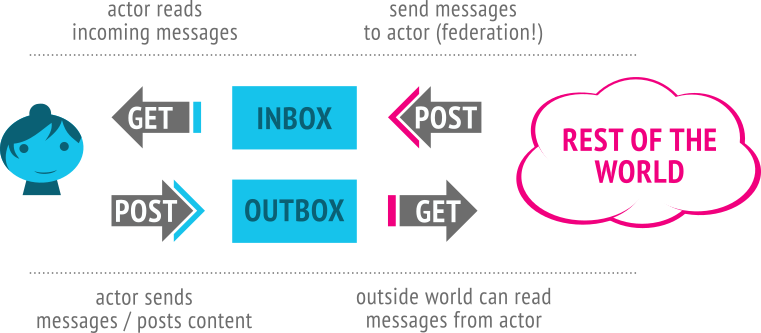
\includegraphics[width=\textwidth]{related_work/ActivityPub-tutorial-image.png}
  \caption{ActivityPub overview \cite{lemmer-webber_tallon_guy_prodromou_2018}}
  \label{fig:ap_flow}
\end{figure}
\pagebreak

Regarding security, ActivityPub's specification does not define any official security mechanisms to ensure confidentiality, non-repudiation, message integrity, authentication, or authorization \cite{lemmer-webber_tallon_guy_prodromou_2018}. However, it mentions a list published by the SocialWG of best security practices\footnote{https://www.w3.org/wiki/SocialCG/ActivityPub/Authentication\_Authorization} that may be used in ActivityPub. This list suggests using standards such as OAuth 2.0\footnote{https://oauth.net/2/} for client-to-server authentication, as well as HTTP Signatures\footnote{https://tools.ietf.org/html/draft-cavage-http-signatures-08} and Linked Data Signatures\footnote{https://w3c-dvcg.github.io/ld-signatures/} for server-to-server authentication. Furthermore, it recommends using HTTPS for its HTTP-based communication to provide at least transport-layer encryption.


% ------------ActivityPub-Based social networks------------------------------------
\section{ActivityPub-based Social Networks}

\subsection{The Fediverse}

It is impossible not to refer to the \emph{Fediverse} when we talk about ActivityPub. The \emph{Fediverse} is an interoperable collection of different federated social networks running on free open software on thousands of servers across the world that implement the same open-standard protocols to be able to interact with each other. In today's most popular social networks like Facebook, Twitter, or Youtube, a centralized architecture keeps millions of users on one platform. Control, decision-making, user data, and censorship depend on a single profit-driven organization. On the contrary, the \emph{Fediverse} is developed by a not-profit-driven community of people around the globe independent of any corporation or official institution \cite{holloway_2018} \cite{https://doi.org/10.48550/arxiv.1909.05801}. The simplest way to explain how the federation works is the following example: Bob has a Twitter account, which he uses to follow all his friends that also have a Twitter account. Alice is a friend of Bob, but she only has an account on Youtube. In the real world, these two services are completely isolated and cannot communicate with each other. However, if both had implemented the same social network protocol, such as ActivityPub, Bob would be able to find Alice by a normal search on Twitter and follow her. Allowing any new post of Alice on Youtube, to appear in Bob's Twitter timeline.

Before ActivityPub, the \emph{Fediverse} implemented other protocols like \emph{Ostatus}\footnote{https://www.w3.org/community/ostatus/wiki/images/9/93/OStatus\_1.0\_Draft\_2.pdf}, \emph{Matrix}\footnote{https://matrix.org}, and \emph{Diaspora}\footnote{https://diaspora.github.io/diaspora\_federation}. However, after ActivityPub was published as a Recommendation by the SocialWG in January 2018, a big number of these federated social networks upgraded to ActivityPub. Becoming rapidly the predominant protocol. Furthermore, the range of services that can be found inside the \emph{Fediverse} includes blogging, microblogging, video streaming, photo, music sharing as well as file hosting. For example: 

\begin{itemize}
  \item \textbf{PeerTube\footnote{https://joinpeertube.org}:} A decentralized alternative to video platforms, similar to Youtube.
  \item \textbf{Mastodon\footnote{https://joinmastodon.org}:} A microblogging social network, similar to Twitter. 
  \item \textbf{Pixelfed\footnote{https://pixelfed.org}:} An image-sharing platform, similar to Instagram. 
\end{itemize} 

Although it was not the first social network to implement ActivityPub, Mastodon is the one that pioneered its use on a large scale \cite{lemmer-webber_2017}. Moreover, it is still the social network in the \emph{Fediverse} with the biggest user base and popularity. For this reason, Mastodon will be used in this thesis as the representative of the ActivityPub-based social networks and will be explained further in the next section. 

% ------------Mastodon------------------------------------
\subsection{Mastodon}\label{subsec:mastodon}

 Mastodon is a decentralized Twitter-like microblogging social network created with the idea to bring social networking back into the hands of its users. The german creator of Mastodon, Eugen Rochko, shared the same opinion as what Fitzpatrick and Recordon said in 2007 \cite{fitzpatrick_recordon_2007}: \emph{People are getting sick of registering and re-declaring their friends on every site}. For this reason, Eugen envisioned a social network that could end this, and \emph{last forever} \cite{tilley_2018}. Similar to the \emph{Fediverse}, Mastodon differs from other commercial social networks in two aspects. First, it is oriented towards small communities and community-based services. Each \emph{instance}\footnote{A server running Mastodon} is free to choose its topics, this way users are encouraged to choose the instance better suited to their taste. Second, the Mastodon platform eliminates the presence of sponsored users or posts in feeds. This implies that the only way to connect or consume content is through a self-search to find an already known account or to explore the feeds of the users in other instances with similar interests \cite{8845221}. From a user experience perspective, Mastodon includes all the essential features of a microblogging platform, such as:

\begin{itemize}
  \item Follow other users, even if they are not in the same instance. 
  \item Post small status updates, or \emph{toots}, up to 500 characters long. 
  \item Access to a timeline of the local instance and federated statuses. 
  \item Control over the visibility of their posts, with the option to set them as private, instance-level only, or federated. 
\end{itemize}

Mastodon's implementation of ActivityPub follows the guidelines defined by the spec. However, the protocol does not specify how to implement some key processes required for a fully-working social network. Therefore, Mastodon extended and complemented the protocol with the following processes and features.


\subsubsection{Security}
Mastodon has implemented the authentication and authorization mechanisms from the best practices list of the SocialWG, to address the security concerns in ActiviyPub. However,  relevant for this thesis are the ones used in federated communication, namely HTTP and JSON-LD Signatures. HTTP signatures extend the HTTP protocol by adding the possibility to cryptographically sign the HTTP requests. This signature gets added to the request within the \emph{Signature} header, and it provides not only end-to-end message integrity but also proof of the authenticity of the sender without the need for multiple round-trips \cite{cavage_sporny_2019}. Creating an HTTP signature means signing the parameters of the request itself, i.e the \emph{request-target}, the \emph{host}, and the \emph{date}. These parameters and their values are concatenated in a single string, hashed, and signed with the sender's public key. Finally, the \emph{Signature} header indicates the key that was used to sign the document, the parameters that are inside the signature, and the algorithm used to hash it. An example in Mastodon is shown by figure \ref{fig:http_signature}. 
Following the same idea, Linked Data Signatures offer a way to create and attach signatures to JSON-LD documents, thus providing non-repudiation to e.g. an ActivityStreams Activity object even if the object has been shared, forwarded, or referenced at a future time \cite{celik_prodromou_le_hors_2014}. However, this feature, although implemented, is not actively used in Mastodon.

\lstset{style=JSONStyle}
\begin{lstlisting}[language=PHP, caption=Signed HTTP Request, label=fig:http_signature, float=h]

GET /users/username/inbox HTTP/1.1
Host: mastodon.example
Date: 18 Dec 2019 10:08:46 GMT
Accept: application/activity+json
Signature: keyId="https://my-example.com/actor#main-key",headers="(request-target) host date",signature="Y2FiYW...IxNGRiZDk4ZA=="

\end{lstlisting}

For Mastodon to be able to implement these signatures, it was necessary to generate keypairs for the users. For this, Mastodon added a new property \emph{publicKey} to the actor object, which includes the pem-formatted public key of an RSA-2018 keypair, as shown in figure\ref{fig:mastodon_actor_object}.

\lstset{style=JSONStyle}
\begin{lstlisting}[language=PHP, caption=Mastodon extended version of ActivityPub's actor object, label=fig:mastodon_actor_object, float=ht]
{
    "@context": [
        "https://www.w3.org/ns/activitystreams",
    ],
    "id": "https://mastodon.social/users/bob",
    "type": "Person",
    "following": "https://mastodon.social/users/bob/following",
    "followers": "https://mastodon.social/users/bob/followers",
    "inbox": "https://mastodon.social/users/bob/inbox",
    "outbox": "https://mastodon.social/users/bob/outbox",
    "featured": "https://mastodon.social/users/bob/collections/featured",
    "featuredTags": "https://mastodon.social/users/bob/collections/tags",
    "preferredUsername": "bob",
    "name": "Bob",
    "summary": "",
    "url": "https://mastodon.social/@bob",
    "manuallyApprovesFollowers": false,
    "discoverable": false,
    "published": "2022-01-18T00:00:00Z",
    "devices": "https://mastodon.social/users/bob/collections/devices",
    "publicKey": {
        "id": "https://mastodon.social/users/bob#main-key",
        "owner": "https://mastodon.social/users/bob",
        "publicKeyPem": "-----BEGIN PUBLIC KEY-----\nMIIBIjANBgkqhkiG9w0BAQEFAAOCAQ8AMIIBCgKCAQEAuWWHabkb/1v/OtK3x3EJ\nvxVaHwwN0PxTbOT/UsDNhu8GynBA2A371rg+BEUFGE/yQ6ljaDcqiQtaAMnuvOpT\nLRUOXu5O5Ct+qBWoLb+Box2NkSWJWc4rP+FXEHM+PTPqJJEplZSKIboCjLijw90V\nCD0hL6nBdXSnNp3CeaiDJfjXx+8MoR7xm4AB4Av0nrrM/eGBd60UM3EqMUVAWYtN\n813hrCmbapi++KY9DE7QpMPUoyOiarvFtl8JpV9HWJ1FrwloT17jJ02smPoCy6iv\nQgDXcAWnMm2PZWuSh/uQ7Y6Iq1ZSCkdQJQwaNsyB6O4BlyPujU2f2wg4nzf5QaBn\nwQIDAQAB\n-----END PUBLIC KEY-----\n"
    },
    "tag": [],
    "attachment": [],
    "endpoints": {
        "sharedInbox": "https://mastodon.social/inbox"
    },
    "icon": {
        "type": "Image",
        "mediaType": "image/jpeg",
        "url": "https://files.mastodon.social/accounts/avatars/107/643/267/140/999/130/original/557f01fa567f8220.jpg"
    }
}
\end{lstlisting}

\subsubsection{Resolving accounts}
As explained in \ref{subsec:ap_workflows}, ActivityPub requires a resolving process when wanting to send a message to a user whose account resides on a different server. For this, Mastodon implemented \emph{Well-Known URIs}\footnote{https://www.rfc-editor.org/rfc/rfc8615.html}, which enable the discovery of information about an origin in well-known endpoints\cite{nottingham_2019}. The two most relevant endpoints are the following: 

\begin{itemize}
  \item \textbf{Web Host Metadata: }
    This endpoint allows the discovery of host information, using a lightweight metadata document format. In this context, \emph{host} refers to the entity in charge of a collection of resources defined by URIs with a common URI host \cite{cook_2011}. It employs the XRD 1.0\footnote{https://docs.oasis-open.org/xri/xrd/v1.0/os/xrd-1.0-os.html} document format, which offers a basic and flexible XML-based schema for resource description. Moreover, it provides two mechanisms for providing resource-specific information, \emph{link templates} and \emph{Link-based Resource Descriptor Documents} (LRDD). On the one hand, link templates require a URI to work, thus avoiding the use of fixed URIs. On the other hand, the LRDD relation type is used to relate LRDD documents to resources or host-meta documents \cite{cook_2011}. In the specific case of the Mastodon implementation, requesting the host-meta endpoint will give us back the \emph{lrdd} link to the Webfinger endpoint, where specific resource information can be found. This is illustrated by figures \ref{fig:host_metadata_response} and \ref{fig:host_metadata_request}.

\lstset{style=JSONStyle}
\begin{lstlisting}[language=PHP, caption=Example Host Metadata request to mastodon.social, label=fig:host_metadata_request, float=ht]
    GET /.well-known/host-meta HTTP/1.1
    Host: mastodon.social
    Accept: application/xrd+xml
\end{lstlisting}

\lstset{style=JSONStyle}
\begin{lstlisting}[language=XML, caption=Example Host metadata response from mastodon.social, label=fig:host_metadata_response, float=h!]
    <?xml version="1.0" encoding="UTF-8"?>
    <XRD xmlns="http://docs.oasis-open.org/ns/xri/xrd-1.0">
      <Link rel="lrdd" template="https://mastodon.social/.well-known/webfinger?resource={uri}"/>
    </XRD>
\end{lstlisting}

\item \textbf{Webfinger:}
Mastodon relies on the Webfinger protocol for the resolving process and its federated functioning \cite{rochko_2020}. Webfinger allows for discovering information about persons or other entities on the Internet using HTTP such as a personal profile address, identity service, telephone number or email. Performing a query to a WebFinger endpoint requires a query component with a resource parameter, which is the URI that identifies the identity that is being looked up. Mastodon employs the \emph{acct}\footnote{https://datatracker.ietf.org/doc/html/rfc7565} URI format, which aims to offer a scheme that generically identifies a user's account with a service provider without requiring a specific protocol. Webfinger's response consists of a \emph{JSON Resource Descriptor} (JRD) Document describing the entity \cite{jones_salgueiro_jones_smarr_2013}. Fig. \label{Webfinger response from mastodon.social} shows an example of the returned JRD document provided by the WebFinger endpoint of the \emph{mastodon.social}\footnote{https://mastodon.social} instance when querying the account \emph{acct:bob@mastodon.social}.

\lstset{style=JSONStyle}
\begin{lstlisting}[language=PHP, caption=HTTP request to Webfinger endpoint, label=Webfinger request, float=h]
  GET /.well-known/webfinger?resource=acct:bob@mastodon.social
  Host: mastodon.social
  Accept: application/xrd+xml
\end{lstlisting}

\lstset{style=JSONStyle}
\begin{lstlisting}[language=PHP, caption=Webfinger response, label=Webfinger response from mastodon.social, float=h]
{
   "subject": "acct:bob@mastodon.social",
   "aliases": [
       "https://mastodon.social/@bob",
       "https://mastodon.social/users/bob"
   ],
   "links": [
       {
           "rel": "http://webfinger.net/rel/profile-page",
           "type": "text/html",
           "href": "https://mastodon.social/@bob"
       },
       {
           "rel": "self",
           "type": "application/activity+json",
           "href": "https://mastodon.social/users/bob"
       },
       {
           "rel": "http://ostatus.org/schema/1.0/subscribe",
           "template": "https://mastodon.social/authorize_interaction?uri={uri}"
       }
   ]
}
\end{lstlisting}
\end{itemize}

\section{Decentralized Identifiers} \label{section:dids}

Globally unique identifiers are used by individuals, organizations, abstract entities, and even internet of things devices for all kinds of different contexts. Nonetheless, the large majority of these globally unique identifiers are not under the entity's control. We rely on external authorities to issue them, allowing them to decide who or what they refer to and when they can be revoked. Their existence, validity scope and even the security mechanisms that protect them are all dependent on these external authorities. Leaving their actual owners helpless against any kind of threat or misuse \cite{sporny_longley_sabadello_reed_steele_2021}. In order to address this lack of control, the W3C DID Working Group conceptualized the Decentralized Identifiers or \emph{DIDs}.

DIDs are a new type of globally unique identifier that enables individuals and organizations to create their own identifiers using trustworthy systems. By means of this, entities are able to prove control over them by authenticating using cryptographic proofs. Furthermore, given that the generation and assertion of DIDs are entity-controlled, an entity can create any number of DIDs that can be tailored and confined to specific contexts. This would enable interaction with other systems, institutions, or entities that require authentication while also limiting the amount of personal or private data to be revealed. All of this without the need to rely on a central authority \cite{sporny_longley_sabadello_reed_steele_2021}. To better illustrate how DIDs work, let's address the components which constitute DIDs. Figure \ref{fig:did_architecture} provides a basic overview of the major components of the Decentralized Identifier architecture.

\begin{figure}[H]
  \centering
  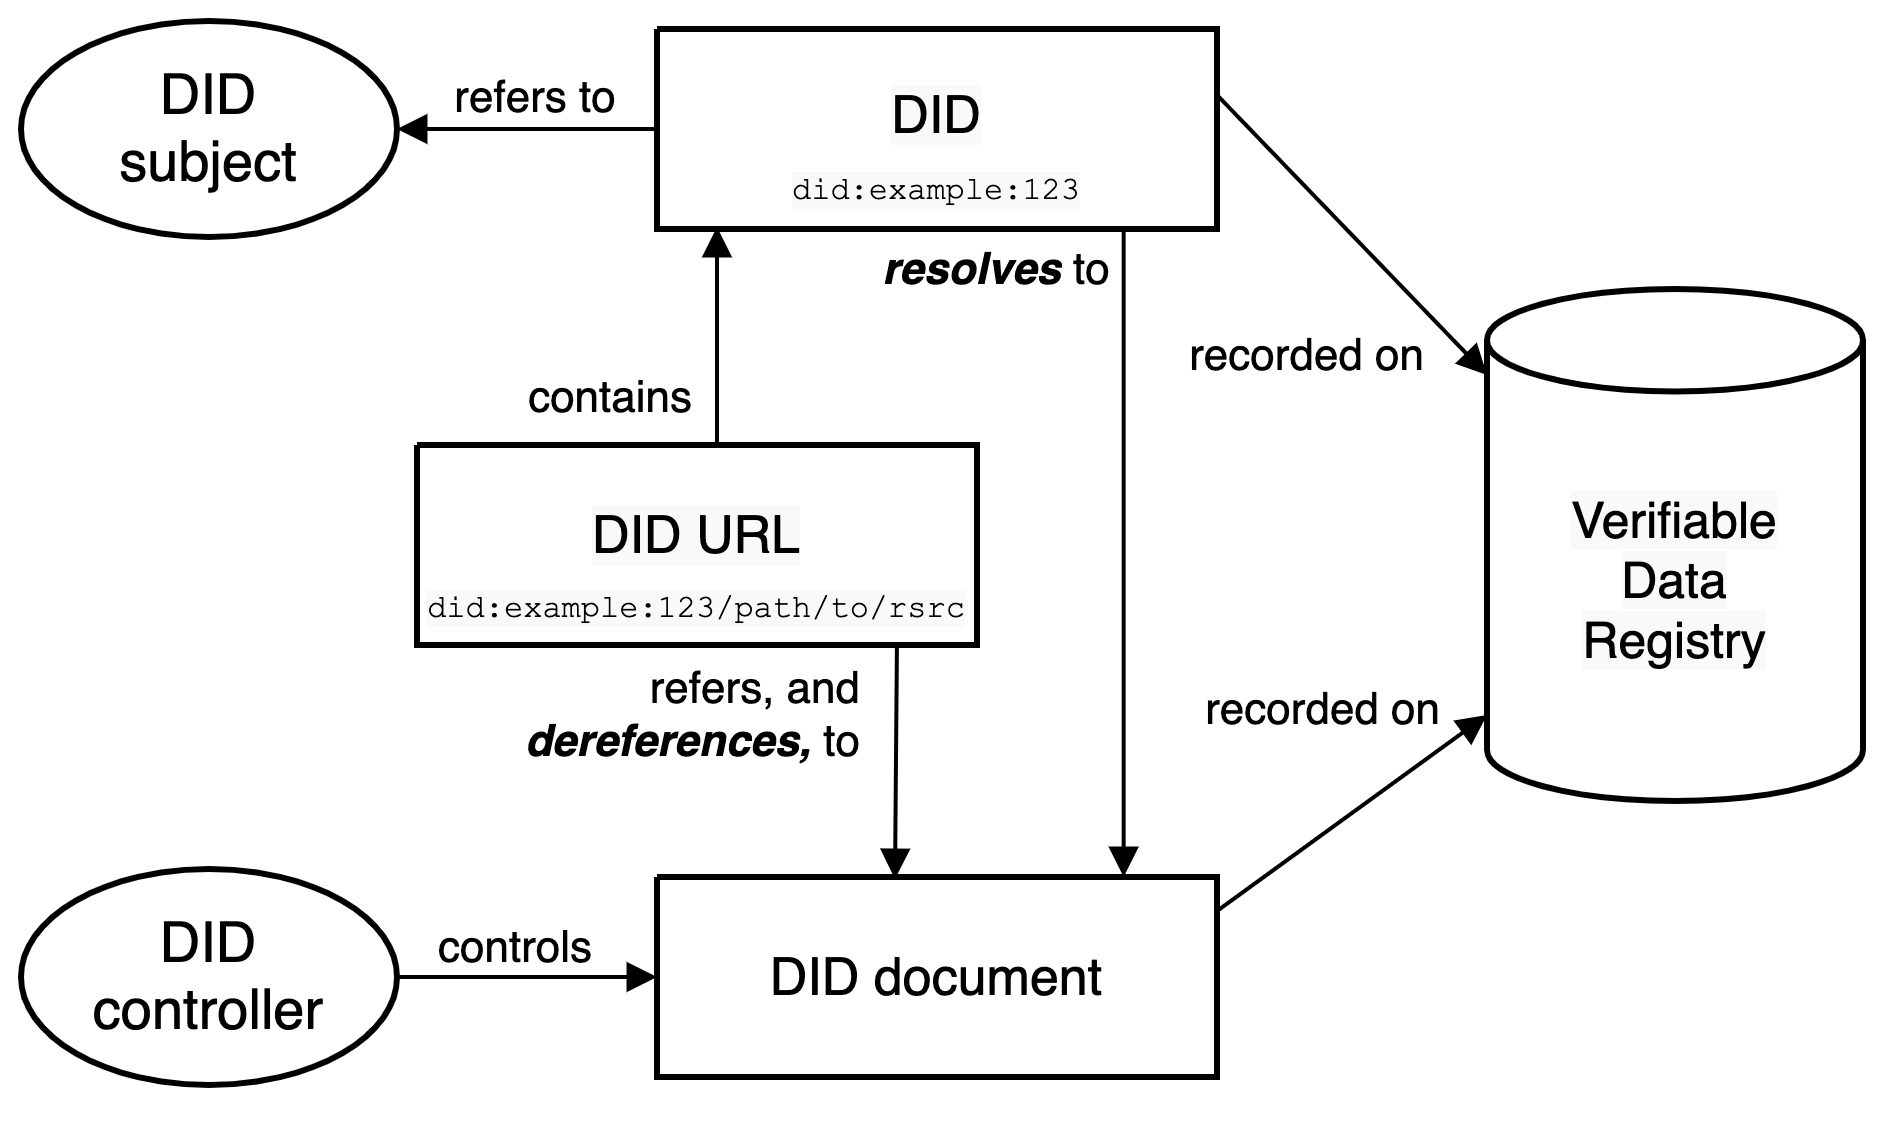
\includegraphics[width=\textwidth]{related_work/did_brief_architecture_overview.png}
  \caption{DID architecture overview \cite{sporny_longley_sabadello_reed_steele_2021}}
  \label{fig:did_architecture}
\end{figure}

\subsection{DID}  
The DID itself is a URI\footnote{https://www.rfc-editor.org/rfc/rfc3986} that consists of 3 different parts, namely the did URI scheme identifier, the method identifier and the DID method-specific identifier.

\begin{figure}[h]
  \centering
  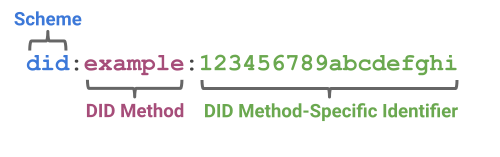
\includegraphics[width=\textwidth]{related_work/parts-of-a-did.png}
  \caption{DID composition \cite{sporny_longley_sabadello_reed_steele_2021}}
  \label{fig:did}
\end{figure}

\subsection{DID URL}

A DID can include a path, query and fragment to be able to locate a specific resource inside a DID document, as shown in \ref{fig:did_architecture}


\subsection{DID Subject}

Refers to the entity being identified by the DID. According to the specification \cite{sporny_longley_sabadello_reed_steele_2021}, any person, group, organization, physical thing, digital thing or logical thing can be a DID Subject.

\subsection{DID Controller}

The DID controller is the entity that can make changes to the DID Document. This entity is not necessarily the DID Subject itself.
  
\subsection{DID Document}

They contain information associated with a DID. They usually describe verification methods, such as cryptographic public keys, as well as services that are relevant to interactions with the DID Subject. An example of a DID Document can be seen in \ref{fig:did_document}.

\lstset{style=JSONStyle}
\begin{lstlisting}[language=PHP, caption=Example DID Document, label=fig:did_document]
{
  "@context": "https://w3id.org/did/v1",
  "id": "did:example:123456789abcdefghi",
  "publicKey": [{
    "id": "did:example:123456789abcdefghi#keys-1",
    "type": "RsaVerificationKey2018",
    "owner": "did:example:123456789abcdefghi",
    "publicKeyPem": "..."
  }],
  "authentication": [{
    "type": "RsaSignatureAuthentication2018",
    "publicKey": "did:example:123456789abcdefghi#keys-1"
  }],
  "service": [{
    "type": "ExampleService",
    "serviceEndpoint": "https://example.com/endpoint/8377464"
  }]
}

% \end{lstlisting}

The only required attribute for a DID Document is the ID. Other optional attributes include a controller, which specifies the DID Controller; verification methods, used to authenticate or authorize interactions with the DID subject or associated parties; and services, which can be any type of service the DID subject wants to advertise, including decentralized identity management services for further discovery, authentication, authorization, or interaction.
 

\subsection{DID methods}

DID methods describe the processes for CRUD operations for DIDs and DID documents, based on a specific type of verifiable data registry. Each DID method describes and implements its own security and privacy considerations. According to the DID registry of the W3C\footnote{https://www.w3.org/TR/did-spec-registries/\#did-methods}, there are around 130 registered DID methods. Based on their characteristics and patterns, the following 4-way classification of DIDs has arisen.

\begin{itemize}
  \item \textbf{Ledger-based DIDs}: This includes all the DIDs that store DIDs in a blockchain or other Distributed Ledger Technologies (DLTs). Examples include did:btcr, did:ethr and did:trx, whose DIDs are stored correspondingly in the Bitcoin, Ethereum and Tron network \cite{preukschat_reed_2021}.
  % \item \textbf{Ledger Middleware ("Layer 2") DIDs}: Broadly speaking, Layer 2 refers to a framework or protocol that is built on top of an existing blockchain system that takes the transactional burden away from layer 1 and post-finalized proofs back to layer 1. By removing this transaction load from layer 1, the base layer becomes less congested, and everything becomes more scalable [https://ethereum.org/en/layer-2/ ]. The Lightning Network ( \, LN	) \, is an example of a layer 2 Bitcoin protocol that offers users a fast micro-payment platform. Furthermore, regarding Layer 2 DID methods, the DIF has developed Sidetree\footnote{https://github.com/decentralized-identity/sidetree}. A protocol for creating scalable blockchain-agnostic Decentralized Identifier networks that enable users to create globally unique, user-controlled identifiers and manage their associated PKI metadata, without the need for centralized authorities or trusted third parties \cite{buchner_steele_ronda_2021}.
  Examples include: did:ion, did:elem.
  \item \textbf{Peer DIDs}: DIDs have the required ability to be resolvable, however not all of them have to be globally resolvable. The DIDs in this category do not exist on a global source of truth but in the context of relationships between peers in a limited number of participants. Nonetheless, their validity is not affected since they comply with the core properties and functionalities that a DID has to provide. 

  \item \textbf{Static DIDs}: This type of DIDs are limited in the kind of operations that can be performed on them. These DIDs are not stored in any registry, consequently, it is not possible to update, deactivate or rotate them. Using the did:key method as an example, the DID-method-specific part of the DID is encoded in a way that the DID document can be deterministically extracted from the DID itself \cite{longley_zagidulin_sporny_2022}.
\end{itemize}


did:ethr
This DID method was registered by Uport, an Ethereum-based system for self-sovereign identity \cite{Lundkvist_Heck_Torstensson_Mitton_Sena_2016}. It allows any Ethereum smart contract or key pair account, or any secp256k1 public key to becoming a valid identifier \cite{nistor_grassberger_carlin_2022}. UPort is a smart-contract-based system that abstracts user accounts using proxy contracts that are held by the user but may be retrieved if keys are lost. To do this, controller contracts create trusted entities for asserting ownership \cite{8783188}


did:ens:
% The Ethereum Name Service (ENS) is a distributed, open, and extensible naming system based on the Ethereum blockchain. Its purpose is to map names like 'bob.eth' into machine-readable identifiers like Ethereum addresses, other cryptocurrency addresses, content hashes, and metadata. In the same way the Domain Name System (DNS) maps human-readable domains like 'google.com' to IP addresses. However, their architecture differs due to the capabilities and constraints of the Ethereum blockchain. (https://github.com/veramolabs/did-ens-spec )
% This DID method was registered by Consensys, a blockchain venture studio founded by Ethereum's cofounder Joseph Lubin that supports Ethereum-based projects. Some of these projects include uPort, Metamask, Civil, Truffle and Gnosis. [https://decrypt.co/resources/consensys]. 


% This DID method was created with the following objectives, firstly to integrate ENS names to be interoperable with applications that implement DIDs, and secondly, to add DID-capabilities to ENS names such as services and verification methods [https://github.com/veramolabs/did-ens-spec].

% did:ion:
% This DID method works by registering DIDs to the Bitcoin network. Launched to the public in March 2021, Identity Overlay Network (ION) is Microsoft's DID-network built on top of the Bitcoin Network implemented using Sidetree (https://techcommunity.microsoft.com/t5/identity-standards-blog/ion-we-have-liftoff/ba-p/1441555 ). 
% ION is public, permissionless, it does not implement its own currency and its nodes do not require an additional consensus mechanism. (https://github.com/decentralized-identity/ion ).

\subsection{Verifiable Data Registry}

Essentially, any system that enables capturing DIDs and returning required data to generate DID documents. This can be distributed ledgers, decentralized file systems, any type of database, peer-to-peer networks, or other types of trustworthy data storage \cite{sporny_longley_sabadello_reed_steele_2021}.

\subsection{DID resolver}

A DID resolver is able to implement the DID resolution, which consists of taking a DID as an input, and giving a DID Document as an output \cite{sporny_longley_sabadello_reed_steele_2021}. As of the writing of this thesis, the Identifiers \& Discovery Working Group (ID WG) has implemented a prototype Universal Resolver\footnote{https://github.com/decentralized-identity/universal-resolver}, which allows the resolution of DIDs for numerous DID methods, including all the examples mentioned above. In addition, this working group has also developed a Universal Registrar\footnote{https://uniregistrar.io/}, which allows the creation, edition and deactivation of the DIDs across different DID methods.

% Comparing DIDs with other identifiers


% UUID Universally Unique Identifiers: 
% UUIDs are similar to DIDs, because they do not require a centralized registration authority. But they are not resolvable or cryptographically-verifiable. 


% Almost all types of identifier systems can support DIDs. This would create an interoperability bridge between centralized, federated and decentralized worlds. Implementers can use any kind of computing infrastructure they trust, such as distributed ledgers, decentralized file systems, distributed databases or peer-to-peer networks. 


% Services
% Services are used to specify ways to communicate with the DID subject. Services can be decentralized identity management for further discovery, authentication, authorization or interaction. 


% DID Privacy 

% The 7 Principles of Privacy by design have been applied to DIDs. (https://iapp.org/media/pdf/resource_center/pbd_implement_7found_principles.pdf )






%  A DID is unlikely to contain any information about the DID subject, so further information about the DID subject is only discoverable by resolving the DID to the DID document, obtaining a verifiable credential about the DID, or via some other description of the DID.



\section{DIDComm Messaging}\label{section:didcomm}

\subsection{Definition}

The Hyperledger Foundation is an open-source collaborative effort intended to further develop blockchain technologies across industries \cite{jones_boswell_2022}. Started in 2016 by the Linux Foundation, it has given birth to numerous enterprise-grade software open-source projects that can be classified into DLTs, libraries, tools and labs \cite{lusard_lehors_muscara_boswell_zsigri_2021}. One of these graduate projects is Hyperledger Aries, which together with Hyperledger Indy (HI) and Hyperledger Ursa (HU), makes up the Sovereign Identity Blockchain Solutions of Hyperledger. HI supplies a distributed ledger specifically built for decentralized identity, HU is a shared cryptography library that helps to avoid duplicating cryptographic work across projects while also potentially increasing security. Finally, Aries provides solutions for SSI-based identity management, including key management, credential management, and an encrypted, peer-to-peer DID-based messaging system that is now labeled as Didcomm v1 \cite{jones_boswell_2022}. 
Based on Didcomm v1, the Communication Working Group (CWG) of the DIF has implemented DIDcomm v2. Among other key differences between versions, such as formalizations of Didcomm v1 methods, Didcomm v2 has removed the special handling of Peer-DIDs in order to make all DIDs equal from the perspective of the DIDComm spec. Furthermore, the CWG pursues the standardization of DIDcomm not only to widen its implementation beyond Aries-based projects but to create an interoperable layer that would allow higher-order protocols to build upon its security, privacy, decentralization, and transport independence in the same way web services build upon HTTP. \cite{young_2020} \cite{curren_looker_terbu_2020}

From this point on, we are going to refer to DIDComm Messaging v2 only as DIDComm. Didcomm can be described as a communication protocol that promises a secure and private methodology that builds on top of the decentralized design of DIDs. Moreover, Didcomm is a very versatile protocol, as it supports a wide range of features, such as security, privacy, decentralization, routable, interoperability, and the ability to be transport-agnostic \cite{curren_looker_terbu_2020}.

To better understand how it works, let's look at how it would work in a scenario where Alice wants to send a private message to Bob: 


% \begin{algorithm}[H]
% \caption{Example of DID communication using DIDComm \cite{Abramson_2020}}
% \label{alg:didcomm_example}
%   \begin{algorithmic}[1]
%     \State Alice has a private key \emph{sk\textsubscript{a}} and a DID Document for Bob containing an endpoint \emph{(endpoint\textsubscript{bob})} and a public key \emph{(pk\textsubscript{b})}.

%     \State Bob has a private key \emph{sk\textsubscript{b}} and a DID Document for Alice containing her public key \emph{(pk\textsubscript{a})}.

%     \State Alice encrypts plaintext message \emph{(m)} using pk\textsubscript{b} and creates an encrypted message \emph{(eb)}.

%     \State Alice signs eb using her private key \emph{sk\textsubscript{a}} and creates a signature \emph{(s)}.

%     \State Alice sends \emph{(eb, s)} to \emph{endpoint\textsubscript{bob}}.

%     \State Bob receives the message from Alice at \emph{{endpoint\textsubscript{bob}}.}

%     \State Bob verifies \emph{(s)} using Alice's public key \emph{pk\textsubscript{a}}

%     \If{Verify \emph{(eb, s, pk\textsubscript{a})} = 1}
%     \State Bob decrypts \emph{eb} using \emph{sk\textsubscript{b}}.
%     \State Bob reads the plaintext message \emph{(m)} sent by Alice
%     \EndIf
%   \end{algorithmic}
% \end{algorithm}


% [https://arxiv.org/pdf/2006.02456.pdf ]

DIDComm differs from the current dominant web paradigm, where something as simple as an API call requires an almost immediate response through the same channel from the receiving end. This duplex request-response interaction is, however, not always possible as many agents may not have a constant network connection or may interact only in larger time frames, or may even not listen over the same channel where the original message was sent. DIDComm's paradigm is asynchronous and \emph{simplex}. Thus showing a bigger resemblance with the email paradigm. Furthermore, the web paradigm goes under the assumption that traditional methods for processes like authentication, session management, and end-to-end encryption are being used. Didcomm does not require certificates from external parties to establish trust, nor does it require constant connections for end-to-end transport-level encryption (TLS). Taking the security and privacy responsibility away from institutions and placing it with the agents. All of this without limiting the communication possibilities because of its ability to function as a base layer where opposed capabilities like sessions and synchronous interactions can be built upon. \cite{curren_looker_terbu_2020}

To achieve the encryption and signing processes mentioned in algorithm \ref{alg:didcomm_example}, Didcomm implements a family of the Internet Engineering Task Force (IETF) standards, collectively called JSON Object Signing and Encryption (JOSE), which will be further explained in the next section. 

\subsection{JOSE Family}

This RFC family includes both the JSON Web Signature (JWS) and the JSON Web Encryption (JWE) standards that are subclasses of the JSON Web Token (JWT), and JSON Web Key (JWK).


The second part of the DIDComm enablement, namely the signing and encrypting, will depend on what kind of security guarantees we want to achieve. DIDComm offers different approaches based on signing and two types of message encryption. Authenticated Sender Encryption (\emph{authcrypt}) and Anonymous Sender Encryption (\emph{anoncrypt}) are both encrypted and delivered to the recipient's DID. Still, they differ because only \emph{authcrypt} gives direct guarantees about the sender's identity. Sending anonymous messages in social networks is not usually the case, and removing the attribution of a post can lead to other problems \cite{martin_2022}. However, social networks like Ask.fm\footnote{https//ask.fm} or NGL\footnote{https://ask.fun} that rely on anonymous posts could use the advantages of \emph{anoncrypt}.

DIDComm recommends using \emph{authcrypt} as the standard to provide confidentiality, message integrity, and authenticity of the sender. For this, \emph{authcrypt} requires the public key authenticated encryption algorithm \emph{ECDH-1PU}\footnote{https://datatracker.ietf.org/doc/html/draft-madden-jose-ecdh-1pu-04}. This algorithm j

This is due to the use of the 
Elliptic-curve Diffie\-Hellman (ECDH) protocol, which allows two parties to build a secure and private channel across an insecure and observable network. This protocol is part of the foundation of popular messaging apps such as Facebook Messenger, Whatsapp, Signal, and Didcomm V1 \cite{shaaban_2021}. This key agreement protocol works by having both parties interchanging the public keys of their EC keypairs and some other public information. Using this public data and their private keys both parties can calculate a shared secret value, which it's the same for both parties. Any other observer or third party is not able to compute this shared secret without the private data \cite{5972416}. 

An alternative to \emph{Authcrypt} that also complies with the required confidentiality and non-repudiation requirements is to have a nested JWT. To achieve this, the plaintext is first signed and then the resulting JWS is used as the payload of a JWE. The algorithm \ref{alg:nested_jwt} illustrates better the workings of this. 

\begin{algorithm}[H]
  \caption{Communication example with nested JWT}
  \label{alg:nested_jwt}
    \begin{algorithmic}[1]
      \State Alice signs a plain text message using her private key \emph{sk\textsubscript{a}} and creates a \emph{(jws)}.
  
      \State Alice encrypts the \emph{(jws)} using Bob's public key pk\textsubscript{b} and creates a \emph{(jwe)}.
  
      \State Alice sends \emph{jwe} to Bob.
  
      \State Bob decrypts \emph{(jwe)} using his private key \emph{sk\textsubscript{b}} and obtains the \emph{jws}
      \State Bob verifies \emph{(jws)} using Alice's public key \emph{pk\textsubscript{a}}
  \end{algorithmic}
\end{algorithm}
  
In both alternatives, the identity of the sender can be confirmed and the plain text message remains encrypted and hidden from any third party that might manage to read the payload. As mentioned in \autoref{section:didcomm}, the JWE can be sent through any unprotected protocol and still keep all of its advantages. 



Compare with other encryption methods. (TLS, Whatsapp end-to-end, Signal) (Use image below)
 

% ---Left out well-known URIs. ----------
% 
% 
% \item \textbf{Change password:}
%   This endpoint origin from the proposal of the Web Application Security Working Group (WebAppSec) of the W3C. It defines a well-known URL that sites can use to make their change password forms discoverable by tools. This URL would enable software, especially password managers, to easily redirect users to the right link for them to change their password \cite{mondello_o'connor_2021}.
% 
%   \item \textbf{NodeInfo: }
%   NodeInfo is an initiative to standardize the presentation of metadata about a server operating one of the distributed social networks. The two main aims are to get greater insights into the distributed social networking user base and to provide tools that allow users to select the most suited software and server for their requirements. Mastodon is one of the implementers of this protocol, along with other federated social networks such as Diaspora, Peertube and WordPress [http://nodeinfo.diaspora.software/ ]. NodeInfo specifies that servers must provide the well-known path /.well-known/nodeinfo and provide a JRD document referencing the supporting documents via Link elements, as shown in \label{NodeInfo response example}. [http://nodeinfo.diaspora.software/protocol.html ] Accessing the hypertext reference from the JRD response will give a schematized series of metadata of the instance running the endpoint, such as NodeInfo schema version, software, protocols supported by the server, statistics and even a list of third-party services that can interact with the server via an API. Figure \label{fig:nodeinfo_response} shows the NodeInfo 2.0 schema of the Mastodon instance mastodon.social. 
% \end{itemize}
% 
% 
% \lstset{style=JSONStyle}
% \begin{lstlisting}[caption=NodeInfo response example, label=NodeInfo response example, float=h]
%   {
%       "links": [
%           {
%             "rel": "http://nodeinfo.diaspora.software/ns/schema/2.1",
%               "href": "https://example.org/nodeinfo/2.1"
%           }
%       ]
%   }
% \end{lstlisting}

% \lstset{style=JSONStyle}
% \begin{lstlisting}[language=PHP, caption=NodeInfo request]
%     GET /wel-known/nodeinfo/2.0 HTTP/1.1
%     Host: mastodon.social
% \end{lstlisting}

% \lstset{style=JSONStyle}
% \begin{lstlisting}[language=PHP, caption=NodeInfo response for mastodon.social, label=fig:nodeinfo_response, float=h]
% {
%    "version": "2.0",
%    "software": {
%        "name": "mastodon",
%        "version": "3.5.3"
%    },
%    "protocols": [
%        "activitypub"
%    ],
%    "services": {
%        "outbound": [],
%        "inbound": []
%    },
%    "usage": {
%        "users": {
%            "total": 718555,
%            "activeMonth": 61717,
%            "activeHalfyear": 178356
%        },
%        "localPosts": 36484017
%    },
%    "openRegistrations": true,
%    "metadata": []
% }
% \end{lstlisting}
\chapter{Concept and Design}
\label{cha:conceptanddesign}
 
The standards presented in Chapter 2 show the potential improvements that can be achieved in key components of ActiviyPub-based social networks such as identity management, discovery, and communication. In this section, we are going to go through the different steps that are required firstly to integrate DIDs into an ActivityPub-based social network, and finally to enable DIDComm Messaging v2 for its communication.

The outline for this chapter is the following. First, individual concepts and definitions of the ActivityPub implementation are introduced and described. Then, an example of a simple use-case in a contemporary ActivityPub server is going to be illustrated and analyzed in order to be able to compare it with section 4.5, which presents the same use-case but with the proposed concept and design that includes DID integration and DIDComm enablement. Consequently, the reasons behind every decision made are going to be detailed in section 4.6, along with comparisons with other non-formalized proposals. 
 
As explained in Chapter 2, Mastodon is the social network that pioneered the use of ActivityPub on a large scale, and it is also the social network with the most active users and presence inside the Fediverse. For this reason, the ideas presented in this section and the modus operandi of the ActivityPub server are going to be scoped to the actual implementation in Mastodon.  
 
 
\section{Definitions}
Mastodon has implemented its own ActivityPub server, and with it also its own terms to express different social network vocabulary. In order to prevent confusion or ambiguities, the used terms in this chapter are explained here. 
 
\begin{itemize}
  \item \textbf{Username}: The username in Mastodon consists of a unique local username and the domain of the instance. Ex. alice@example.com
  \item \textbf{Actor object}: In this section, the term Actor object refers solely to the ActivityPub's actor object explained in Chapter 2. 
  \item \textbf{Toot}: In the user-facing part of Mastodon, a Toot is the äquivalent of a Tweet in Twitter. This is a small status update with a 500 character limit.
  \item \textbf{Status}: In the backend of Mastodon, the descriptor used for a Toot is a Status. Moreover, an account in Mastodon has a 1:n relationship with status.
\end{itemize}

\section{Use case}
In order to explain the current ActivityPub flow in Mastodon, let's describe what happens in the simple use case:

\emph{Alice has an account in the Mastodon instance mastodon.social and follows Bob, who has an account in the Mastodon instance mastodontech.de. Alice sends a direct message to Bob with the text: "Hello Bob!" }

\section{Today's implementation}

\begin{figure}[h]
  \centering
  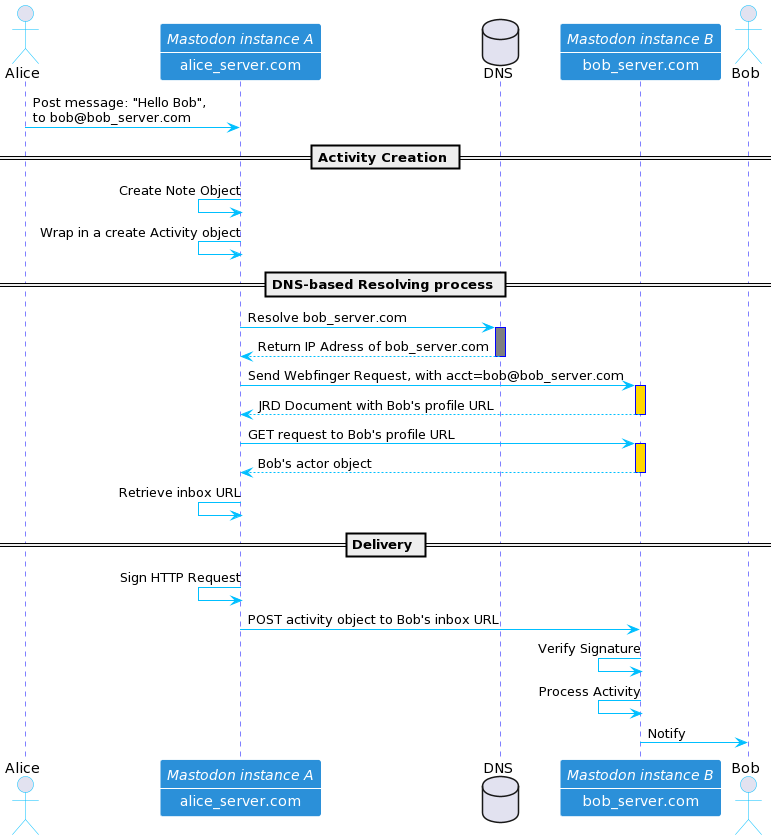
\includegraphics[width=\textwidth]{concept_and_design/normal_flow.png}
  \caption{Current flow for sending message}
  \label{fig:normal_flow}
\end{figure}

\subsection{Object creation}
The first thing that happens when Alice presses the send button is the creation of an ActivityStreams object. In this case, the object is of type \emph{Note}, and will be created by the ActivityPub server inside the Mastodon instance, as shown in \ref{fig:create_note}. Then, following the ActivityPub pattern of \emph{some activity by some actor being taken on some object}, the server wraps it in an ActivityStreams \emph{Create} activity, which contains Alice as the actor. This is illustrated by \ref{fig:create_activity}. Now that the actor, the activity, and the object are well defined and wrapped, it is time to shift our focus to the recipients of this note object. 
The ActivityPub server will now look at all the fields of the ActivityStreams \emph{Audience}, which includes: to, bto, cc, bcc, and audience \cite{snell_prodromou_2017}, where all the addresses of the recipients can be retrieved. Afterwards, depending on where the recipient's account lives, the ActivityPub server may take one of two options. Even though the use-case explicitly dictates that Bob's account resides in a different Mastodon instance, both cases will still be explained.

% Note Object with content: 'Hello Bob'
\lstset{style=JSONStyle}
\begin{lstlisting}[language=PHP, caption=JSON example]
{
	"a":	1,
	"b":	"2",
	"c":	true
}
\end{lstlisting}

\lstset{style=JSONStyle}
\begin{lstlisting}[language=PHP, caption=ActivityStreams note object, label=fig:create_note]
  {
    "@context": "https://www.w3.org/ns/activitystreams",
    "type": "Note",
    "to": "http://bob_server.com/users/bob",
    "attributedTo": "http://alice_server.com/users/alice",
    "content": "Hello Bob!"
  }
\end{lstlisting}

\lstset{style=JSONStyle}
\begin{lstlisting}[language=PHP, caption=ActivityStreams create activity, label=fig:create_activity]
  {
    "@context": "https://www.w3.org/ns/activitystreams",
    "type": "Create",
    "id": "https://alice_server/users/alice/statuses/634367/activity",
    "to": "http://bob_server.com/users/bob",
    "actor": "http://alice_server.com/users/alice",
    "object": {
      "type": "Note",
      "to": "http://bob_server.com/users/bob",
      "attributedTo": "http://alice_server.com/users/alice",
      "content": "Hello Bob!"
    }
  }
\end{lstlisting}


\subsection{Same-server delivery}
If the recipient's account is on the same server, there is then no explicit discovery process. A simple query in the ActivityPub's server would find the right account and save the status within the account's statuses. 


\subsection{Discovery}
On the contrary, when the recipient's account is not in the same server, then a discovery process must be started. Discovery is the fundamental part of the federated side of Mastodon. Without it, users within different instances would not be able to interact, as the instance itself does not know where to find the actor object with all required endpoints to send or receive activities from and to external accounts. For this reason, the current way to look up for other accounts is through the DNS. In the same way Email works, the domain part of the username in Mastodon points to the domain of the instance where the account lives. The purpose of the discovery in this specific use-case is to find the inbox url of Bob, which can can be found in Bob's actor object. As explained in \autoref{cha:relatedwork}, Mastodon includes a series of well-known endpoints that are used to retrieve information about the host itself, as well as resources or entities that are managed under the same host.By default, when the account is not found on the same server, a Webfinger query is performed. 
In our case, Bob's account lives inside \emph{bob\_server.com}. The request shown in \ref{fig:webfinger_request} will return a JRD Document, as shown in fig. \ref{fig:jrd_document}. Based on this document, the Mastodon instance retrieves the link with the \emph{rel: 'self'} which includes the type and the href where the Bob's actor object can be retrieved. If the Webfinger request returns a 404 code, it will then try, as a fallback, using the Host-Meta endpoint. The request and response are displayed in \ref{fig:hostmeta_request} \ref{fig:hostmeta_response}. If successful, it will then proceed to take the link template provided and try the Webfinger request once more before throwing an error. After retrieving the needed URL, a subsequent HTTP GET request to this endpoint with the specific \emph{application/activity+json} header will resolve Bob's actor object. 

\begin{lstlisting}[language=PHP, caption=Webfinger request, label=fig:webfinger_request]
  GET /.well-known/webfinger?resource=acct:bob@bob_server.com HTTP/1.1
  Host: bob_server.com
  Accept: application/ld+json
\end{lstlisting}

\lstset{style=JSONStyle}
\begin{lstlisting}[language=PHP, caption=JRD Document, label=fig:jrd_document, float=h]
  {
    "subject": "acct:bob@bob_server.com",
    "aliases": [
      "https://bob_server.com/@bob",
      "https://bob_server.com/users/bob"
    ],
    "links": [{
        "rel": "http://webfinger.net/rel/profile-page",
        "type": "text/html",
        "href": "https://bob_server.com/@bob"
      },
      {
        "rel": "self",
        "type": "application/activity+json",
        "href": "https://bob_server.com/users/bob"
      },
      {
        "rel": "http://ostatus.org/schema/1.0/subscribe",
        "template": "https://bob_server.com/authorize_interaction?uri={uri}"
      }
    ]
  }
\end{lstlisting}

\begin{lstlisting}[language=PHP, caption=Hostmeta request, label=fig:hostmeta_request, float=h]
  GET /.well-known/host-meta HTTP/1.1
  Host: bob_server.com
  Accept: application/xrd+xml
\end{lstlisting}

\lstset{style=JSONStyle}
\begin{lstlisting}[language=PHP,caption=Hostmeta response, label=fig:hostmeta_response, float=h]
  <?xml version="1.0" encoding="UTF-8"?>
  <XRD xmlns="http://docs.oasis-open.org/ns/xri/xrd-1.0">
      <Link rel="lrdd" template="https://bob_server.com/.well-known/webfinger?resource={uri}"/>
  </XRD>
\end{lstlisting}


\subsection{Delivery}
Succeeding the retrieval of Bob's actor object and therefore the needed inbox URL, a delivery can now take place. In this case, an HTTP POST request with the previously generated activity object. In order to provide end-to-end message integrity and to authenticate Alice in Bob's server, the request is signed by Alice's ActivityPub server using the HTTP Signature specification.
Finally, upon receiving the POST request to Bob's inbox URL, Bob's server verifies the validity of the signature using Alice's public key. After a successful validation, it saves the Note object in Bob's statuses. 

As indicated in chapter 2, HTTP signatures are not part of the ActivityPub protocol standard. These integrity and authentication features are within the Mastodon implementation of an ActivityPub server.


\section{Proposed implementation}
Proposed implementation
Having seen the current flow of our use case mentioned above in a working ActivityPub-based social network, this section will now address the first research question of this bachelor thesis. That is, the implications of integrating DIDs to a Mastodon instance, and therefore to ActivityPub. 

\subsection{Implications of integrating DIDs}
As mentioned in the definitions section, Mastodon's full username includes the domain of the server, and a locally-unique username. This type of username accomplishes the goals of human-readability and uniqueness. In addition, they are resolvable using DNS and the discovery methods previously mentioned in section \autoref{cha:relatedwork}. An ActivityPub actor object using such a username is shown in \ref{fig:alice_actor_object}.  

% Even though there are cases when very similar domains may lead to confusion and may present some security issues. Examples of this can be found simply by comparing the most used Mastodon instance “mastodon.social” with another big-in-user-count instance such as “mstdn.social”. This type of username allows the following scenarios to play out, where differences are minimal and easily missed out, such as alice@mastodon.social and alice@mstdn.social. In addition, some users have commented that when the username is too long, the domain is not longer visible. This can be exploited by malicious actors, who may open an account in a different server with the same username as their target. Clone their profile, and try to social engineer the target's followers. 

\lstset{style=JSONStyle}
\begin{lstlisting}[language=PHP, caption=Alice's actor object, label=fig:alice_actor_object, float=h]

{
	"@context": [
			"https://www.w3.org/ns/activitystreams",
			"https://w3id.org/security/v1",
	],
	"id": "http://alice_server.com/users/alice",
	"type": "Person",
	"following": "http://alice_server.com/users/alice/following",
	"followers": "http://alice_server.com/users/alice/followers",
	"inbox": "http://alice_server.com/users/alice/inbox",
	"outbox": "http://alice_server.com/users/alice/outbox",
	"featured": "http://alice_server.com/users/alice/collections/featured",
	"featuredTags": "http://alice_server.com/users/alice/collections/tags",
	"preferredUsername": "alice",
	"name": "",
	"summary": "",
	"url": "http://alice_server.com/@alice",
	"manuallyApprovesFollowers": false,
	"discoverable": false,
	"published": "2022-06-14T00:00:00Z",
}


\end{lstlisting}

The first question that needs to be addressed when approaching the integration of DIDs to Mastodon and therefore ActivityPub is, what are the implications of switching from standard mastodon usernames to DIDs. Integrating DID to ActivityPub points immediately to the actor's object. Making the switch would mean that the DID has to be included. Currently, most of the interactions of the ActivityPub server inside Mastodon require the ID attribute to resolve to the Actor's profile and thus the Actor's object. Following a simple strategie, we could simply replace the username with the DID. Thus having an ID attribute that may look like this: 

% \emph{id: www.alice_server.com\/users\/did\:example\:123456789abcdefghi }


% However, there is another alternative that might work. Following the ActivityPub's  specification, the ID attribute must be a publicly dereferencable URI, whose authority belongs to the originating server \cite{lemmer-webber_tallon_guy_prodromou_2018}. As explained in section(DID number), a DID is a URI and it is publicly dereferencable by nature. This allows different possibilities, in which the DID can be added. Take for example, using a stand-alone DID as an ID attribute, in order to take advantage of the discoverability of DIDs. This scenario would have the following implications. If another ActivityPub Server wanted to simply get the actor's profile URL, it would require resolving the DID to its respective DID-Document, adding the need to parse it and to methodically do a search until the endpoint is found and retrieved. This additionally requires that the DID-Document includes the actor's profile in the services section. This modification in the DID Document will be further discussed in the Discovery section. Moreover, another option would be to add a DID-URL with a query that points directly to the service endpoint that contains the actor's profile URL. Simplifying in this manner the work that the ActivityPub server must do, although  still requiring a DID resolution as an intermediate step, as well as adding the service endpoint to the DID-Document. Both cases are possible, because ActivityPub has the URL attribute that requires the actor's profile URL in case that it is not in the ID attribute \cite{lemmer-webber_tallon_guy_prodromou_2018}. Although plausible, for the purpose of this Thesis we will keep a simple replacing strategie and keep the ID attribute as the profile's URL with the username replaced with the DID. 

DID URLs provide a lot of freedom of usability for DIDs. In addition to the ID, the actor's object must provide a supplementary set of URLs that point to different collections related to the Actor. These include mandatory attributes, like the outbox and the inbox, and other optional attributes such as the followers and following attributes. What if, instead of using the actual URL of these collections, we specify DID URLs that then point to the correct endpoint inside the DID-Document. This example is illustrated in fig. (Activitypub actor with all DID URLS). 


% This approach leads us to the question, isn't it simpler just to shift the whole actor's object endpoints directly to the DID-Document? Therefore removing the need for an ActivityPub actor's object. This idea was briefly suggested by \cite{webber_sporny_2017} in a paper prepared for the 2017 Rebooting Web of Trust summit. Such an idea would look like (fig. DID-Document with all ActivityPub endpoints). Furthermore, the authors went a step further and proposed cutting all dependency from the DNS by using onion websites. The authors however failed to offer an adequate explanation and consideration of the ActivityPub protocol in existing implementers. Moreover, there are some security privacy concerns regarding the use of service endpoints in the DID Document. The DID specification stipulates "revealing public information through services, such as social media accounts, personal websites, and email addresses, is discouraged" \cite{sporny_longley_sabadello_reed_steele_2021}. DID Documents are stored in a publicly available verifiable data registry, therefore any personal information revealed here is for everyone to see. The usage of URLs in service endpoints might lead to involuntary leakage of personal information, or correlation between the URL and the DID subject. Looking at Fig(fig. DID-Document with all ActivityPub endpoints), the amount of personal information displayed in the DID Document, which would not be otherwise inferable, already poses a privacy issue for the DID Subject. For this reason, in this thesis we differ from removing the actor's object from the ActivityPub protocol itself. This would also allow us to use freely all the other attributes in the actor's object to further describe its owner, such as name, preferredUsername, or summary without making this information forever public in an immutable ledger. Fig(final Actor'S object) illustrates the final design for the DID-compliant actor object. 
% Regarding Mastodon, replacing the standard username with a DID does not imply huge complications. When creating a username there are some validations made to it, such as length, regex and uniqueness. All of this is contained inside the Account class, which is the object that abstracts all a user's account. An example of the Mastodon instance that uses DIDs instead of standard usernames is illustrated in fig. (Image of Mastodon with DIDs). 


% Discovery
% As stated in the previous section, Mastodon starts the discovery process based on the username of the user. By replacing the standard username with a DID, the current discovery flow gets disrupted, as there is no domain and thus no well-known endpoints to send discovery requests to. Nonetheless, here is where the discoverability and always resolvability of the DIDs comes into play. The proposed flow of discovery takes the following steps. Firstly, the username, which now is a DID, can be resolved to its DID-Document using any kind of DID resolver. An example can be the Universal Resolver from the DIF mentioned in Chapter 2. The DID Document must now contain a service section with the type ActivityPub and a URL, where the actor's object can be retrieved. This gives us 2 possibilities. One the one hand, we could add in the well-known Webfinger endpoint, which then provides us with the profile URL from the user. On the other hand, we could skip the Webfinger request and provide the profile URL directly in the DID-Document. The latter looks like the most meaningful path to take. Especially when we refer to the purpose of Webfinger, which was to enable discoverability of entities represented by URIs [https://webfinger.net/ ]. Webfinger's purpose shares a lot of ground with the discoverable design of DIDs, nevertheless the DID design provides a less limited structure of discovery, as it does not rely on DNS and HTTP for its functioning. For this reason, the proposed workflow will completely remove the use of the discovery protocol Webfinger used in Mastodon and include the URL of the actor's profile in the ActivityPub service section in the DID Document. 

% \subsection*{Enabling DIDComm Messaging}

% Considering the fact that DIDs are now implemented in our ActivityPub prototype, it is now possible to enable the DIDComm messaging protocol. Taking into account the algorithm shown in the DIDComm section, it is possible to derive some requirements that DIDComm imposes: 

% DID-Documents may present more than one verification method specified in them. A specific standard verification method is required in order to maintain compatibility between the parties involved. This means that the sender and the recipient must use the same set of keys for encryption and or signing purposes to have a successful message exchange through DIDComm. The DID specification luckily provides us with a recommendation for this. The keyAgreement verification relationship is intended to provide the keys, which allows an entity to confidentially share information with the DID-subject using encryption. (DID-core) Even though it is possible to add an extra verification relationship called DIDComm or ActivityPub that works in conjunction with our previously defined ActivityPub service, we will stick to the recommendation of using the keyAgreement key for our proposal.

% The ActivityPub server requires access to the private key of the selected verification method. This of course imposes risks, as the private key is no longer in the user's control. The administrator of the Mastodon instance would have access to the plain-text private key, and some security countermeasures like key rotation would not be able to counter this. Furthermore, the ActivityPub server must be able to support the keys and the cryptographic algorithms, which the JWA includes. This means having any kind of library that is able to parse them and perform encryption as well as decryption with them. 

% Finally, the ActivityPub server must have access to a DID resolver, in order to retrieve DID-Documents. Especially in cases where an incoming message has been signed, and the signature needs to be verified using a specific public key. This requires extending the Mastodon server by adding possibly a service class that can perform calls to a DID-resolver and parse the returned DID-Document in order to process the information in it. 
% ActivityPub encapsulation
% As part of this proposal, we do not want to do further changes to the ActivityPub protocol itself. However, extending it and removing the dependency to the HTTP protocol for its communication is still intended. Therefore, encapsulation rather than modification of ActivityPub within DIDComm allows for a modular approach that keeps both protocols independent from each other. DIDComm presented 3 different kinds of message structures, namely plain text (JWM), signed (JWS) and encrypted messages (JWE). The following sections present how the encapsulation, as well as signing and encryption processes work in this proposal.

% ActivityPub as JWM
% Let's take our previous example of an ActivityStreams object where Alice sends a message to Bob. The simplest way to keep a modular approach is by using the ActivityStream object as payload for our JWM, which would look like fig. (JWM with activity). As explained in chapter 2, the JWM specification defines a series of attributes that provide a starting point for the use of JWMs. Not all of these are mandatory and can thus be modified depending on the use being given to them. This gives us a lot of room to think what is actually necessary and what is not. As seen in fig. (JWM with activity), redundancy can be found in each level of the json object. For example, the sender and recipient are being defined in each layer. At the end, the object that is going to be processed is the Activity. The JWM does not necessarily need any extra information, because the Activity already has everything. The following table shows a mapping from the JWM attributes to the ActivityStreams object, proving that redundancy can be removed. 

% From => attributedTo
% To: => To 
% Expires_time => Not needed, statuses do not expire
% Created_time => published

% Furthermore, even if we wanted to use the routing mechanism of DIDComm, the attributes From and To in the JWM would only be necessary in cases where we want to send plain text messages. In addition, in almost every case the message is being sent to a specific URL, like the inbox of another user. So the receiver will always know to whom the Activity was directed.
% This leaves us with a JWM structure with the attributes id and type. The requiredness of these two differs from the JWM specification and DIDComm. Nonetheless, we will stick to DIDComm and make these two attributes compulsory. The type should be a message type URI, therefore we will use the ActivityStreams schema URI, and for the ID, we will reuse the status ID. The end result  is shown by fig. (COMPLETE JWM)

% {
%   "id": "https://some.activitypub.server/moriel/posts/a29a6843-9feb-4c74-a7f7-081b9c9201d3",
%   "type": "https://www.w3.org/ns/activitystreams",
%   "body": {
%     "message": {
%       "@context": "https://www.w3.org/ns/activitystreams",
%       "type": "Create",
%       "id": "https://mastodon.example/users/alice/statuses/...",
%       "actor": "https://mastodon.example/users/alice",
%       "to": [ 
%             "bob@chatty.social"
%         ],
%       "object": {
%         "type": "Note",
%         "to": [ 
%             "bob@chatty.social"
%         ],
%         "attributedTo": "https://mastodon.example/users/alice",
%         "content": "Hello Adrian!"
%       }
%     }
%   }
% }

% The second part of the DIDComm enablement, namely JWS, JWE or both, will depend on what kind of security guarantees we want to achieve. The DIDComm specification offers different approaches [foot note: https://identity.foundation/didcomm-messaging/spec/#iana-media-types], based on signing and two types of message encryption, Authenticated Sender Encryption ("authcrypt") and Anonymous Sender Encryption ("anoncrypt"). Both forms are encrypted and delivered to the recipient's DID but they differ in the fact that only authcrypt gives direct guarantees about the sender's identity. Sending anonymous messages in social networks is not usually the case, and in some cases it can lead to other problems like increased cyberbullying and harassment when attribution is removed [https://www.forbes.com/sites/iainmartin/2022/06/29/hugely-popular-ngl-app-offers-teenagers-anonymity-in-comments-about-each-other/?sh=38a95a5153d1]. However, some social networks like Ask.fm [footnote], Whisper or NGL Q&A that rely on anonymous posts could use the advantages of anoncrypt. Therefore for our Mastodon case, we will focus on the use cases with authcrypt. As signing a message brings different guarantees than encrypting a message, we will next look at both JWS and JWE advantages, to deliberate which use cases best apply to them. 


% JWS provides on the one hand non-repudiability, authenticity and integrity to a JWM, and its origin can be thus proven to any external party. Sending DIDComm messages as a JWS, would be the equivalent of the currently used HTTP and Linked data Signatures in Mastodon. 
% On the other hand, JWE provides 


% @startuml
% actor Alice as a
% participant Alice_Server as as
% database VDR
% participant Bob_Server as bs
% actor Bob as b

% a->as: Message to Bob: "Hello Bob!"
% as<-as: Create Note Object
% as<-as: Wrap object in Activity
% as<-as: Sign using Alice's private key

% == Discovery ==
% as->VDR ++ #gray: Resolve Bob's DID
% VDR-->as --: Bob's DID Document
% as<-as: Retrieve service endpoint \n url and public_key 
% as<-as: Encrypt using\nBob's public Key

% as->bs ++ #gold: GET service endpoint url
% bs-->as --: Bob's actor Object
% as<-as: Retrieve inbox url

% == Delivery ==
% as->bs: POST encrypted message

% bs<-bs: Decrypt using Bob's\nprivate key
% bs->VDR ++ #gray: Resolve Alice's DID
% VDR-->bs --: Alice's DID Document

% bs<-bs: Retrieve public_key 
% bs<-bs: Verify Signature

% bs->b: Notify
% b<-b: Read Message

% @enduml


% @startuml
% actor Alice as a
% participant Alice_server as as
% database DNS
% participant Bob_server as bs
% actor Bob as b

% a->as: Post message: "Hello Bob!"
% as<-as: Create Note Object
% as<-as: Wrap object in Activity

% == Discovery ==


% as->DNS ++ #gray: Resolve Bob's server domain
% DNS-->as --: Return IP Adress of bob-server.com

% as->bs ++ #gold: Send Webfinger Request
% bs-->as --: JRD Document describing Bob
% as<-as: Retrieve Bob's \nprofile url

% as->bs ++ #gold: GET user profile url
% bs-->as --: Bob's actor object
% as<-as: Retrieve inbox \nurl

% == Delivery ==
% as->bs: POST message to Bob's inbox url

% bs->b: Notify

% b<-b: Read message

% @enduml
\chapter{Implementation}
\label{cha:implementation}

The source code of this thesis prototype is available on GitLab and can be accessed under the following link: \verb|https://gitlab.com/Lisztos/mastodon|. It was implemented using two different Mastodon instances. The first one was a Linux server with Ubuntu 20.04, 2 CPU cores,  4GB RAM, and 80 GB storage capacity provided by the cloud provider Linode\footnote{https://linode.com}. The TU Berlin provided the second one, which was mainly used for debugging requests and testing the resolving processes in federated communication. Both domains used for the servers are \emph{lisztos.com} and \emph{tawki.snet.tu-berlin.de}. Amazon Simple Email Service (SES) was selected as the email delivery service, and Amazon S3 was used for storing the profile images of the servers. 

\section{Mastodon}

The source code\footnote{https://github.com/mastodon/mastodon} of Mastodon is open source and accessible for everyone to download. The core backend was implemented using the Model-View-Controller framework Ruby on Rails\footnote{https://rubyonrails.org/}, based on the Ruby programming language. The backend manages a Postgres\footnote{https://www.postgresql.org/} database, implements the ActivityPub server, provides a REST API for the frontend, and serves some web pages. The frontend of Mastodon was complemented using the React\footnote{https://reactjs.org} framework, which manages most of the dynamic parts of the interface. Finally, Nginx serves as the reverse proxy for the Mastodon instance.  
Mastodon provides a docker-compose configuration file to facilitate the deployment process. However, it was extended with the DID resolver services for the prototype. The services inside the extended docker-compose file are described in table \ref{table:mastodon_service}.

\begin{table}[H]
  \centering
  \begin{tabular}{|p{4cm}|p{10cm}| }
    \hline
    Service name & Description \\
    \hline
    \hline
    Web & Mastodon Rails application \\
    \hline
    DB & Postgres database \\
    \hline
    Redis & In-memory data store for caching and streaming \\
    \hline
    ElasticSearch (es) & Search engine for accounts or tags\\
    \hline
    Streaming & Mastodon's React application \\
    \hline
    Sidekiq & Tool to perform asynchronous processing\\
    \hline
    DID Resolver & Service to resolve DIDs \\
    \hline
    Uni-resolver-driver-did-uport & Driver for the did:ethr method\\
    \hline
  \end{tabular}
  \caption{Mastodon services}
  \label{table:mastodon_service}
\end{table}

\subsection{Requirements}

The requirements to run a mastodon server are:
\begin{itemize}
  \item Ubuntu 20.04 or Debian 11 for the operating system
  \item Domain name
  \item Email delivery service
  \item Object storage service (optionally)
\end{itemize}

Software requirements include: 
\begin{itemize}
  \item Nginx
  \item Docker
  \item Docker-Compose
\end{itemize}


\subsection{Configuration}

For external configuration, it is required that the domain name points to the IP address of the server. Furthermore, the accounts and providers for the Email delivery service or the object storage service must be set up in advance. 
Additionally, Nginx\footnote{https://nginx.com} is used to serve the Mastodon instance. Unfortunately, Nginx was not containerized and it must be manually configured. For complete instructions to configure Nginx see appendix \ref{appendix:nginx_configuration} 


\subsection{Build}

To build the source code of the prototype it is first required to add an \emph{env} file with the necessary environment variables for development to the root folder. An example file can be found in appendix \ref{appendix:env_file}, however, it is necessary to fill it up with the required credentials. Next, the image from the web service needs to be manually built with the following command. The \emph{-f} flag specifies to use the custom \emph{Dockerfile} and the \emph{-t} flag adds a name and tag to the image. 
  
\lstset{style=CodeStyle}
  \begin{lstlisting}[language=PHP, caption=Building the development Dockerfile, float=h]
    docker build -f Dockerfile.dev -t mastodon:dev .
  \end{lstlisting}


\subsection{Run}
After building the development image for the rails application, it is now possible to pull the images for the other services from the docker registry and get every container running using the commands shown in listing \ref{list:start_mastodon}.

\lstset{style=CodeStyle}
\begin{lstlisting}[language=PHP, caption=Starting all services of Mastodon, label=list:start_mastodon, float=ht]
  // Create and start containers
  docker-compose up -d

  // Restart NGINX
  sudo systemctl restart nginx

  // When everything is running, we need to run the migrations
  docker-compose exec web rails db:migrate
\end{lstlisting}


Visiting the provided domain using HTTPS will show the welcome page of Mastodon. In order to test the federated communication, this process should now be repeated using a different server. Having two different domain names was required for the prototype to test the whole DNS-based resolving process. However, the setup might also work using the raw IP address as the default domain. 


\section{DIDs}

In order to create a DID, the source code of the prototype includes a \emph{/veramo\_agent} folder with all the needed methods to perform CRUD operations to DIDs from the \emph{did:ethr} method. The setup was taken from Veramo's guides\footnote{https://veramo.io/docs/node\_tutorials/node\_setup\_identifiers/}, and the methods for the CRUD operations were written based on the API reference \footnote{https://veramo.io/docs/api/core}. 

\subsection{Requirements}

Software requirements to build the Veramo agent include: 
\begin{itemize}
  \item Node v14+
  \item Yarn
\end{itemize}

\subsection{Configuration}
First, an \emph{.env} file that contains the variable: \emph{INFURA\_PROJECT\_ID="example-infura-project-id"} from an Infura\footnote{https://infura.io/} account is required. This project ID has to match the Ethereum network desired. The default selected in the setup is \emph{Ropsten}.

\subsection{Build}
To build the project, the only command needed is \emph{yarn install} in the root of the \emph{/veramo\_agent} folder. 

\subsection{Run}
A set of \emph{scripts} are provided to facilitate the use of the CRUD methods. See table \ref{table:yarn_scripts} for a detailed view. However, to make any changes to a DID, it is first necessary to fund the Ethereum account to which the DID is anchored. This account can be found in the DID document, with the key \emph{blockchainAccountId} of the first verification method, as shown in listing \ref{fig:blockchain_id}. It follows the format  \emph{eip155:<network id>:<0x ethereum address>}. If the DID was created using a test network, the address can be funded using any Faucet\footnote{https://faucet.egorfine.com/}. Otherwise, Ether has to be transferred from a real account.
Finally, the prototype only supports parsing RSA keys from the DID document. To further understand how adding an RSA key works in Veramo, please refer to:\\
 \verb|https://gist.github.com/Lisztos/eade1f9199d46392f7c7d1f9bbfe7a3b|


\begin{table}[H]
  \centering
  \begin{tabular}{|p{4cm}|p{3cm}|p{7cm}| }
    \hline
    Command & Parameters & Description \\
    \hline
    \hline
    yarn id:create & & Creates a new DID \\
    \hline
    yarn id:list & & List the created identifiers by this agent \\
    \hline
    yarn id:resolve\_did & DID & Resolved the DID to its the DID document \\
    \hline
    yarn id:add\_service & DID,  Service \ref{fig:service_object} & Adds a new service to the DID document \\
    \hline
    yarn id:remove\_service & DID, Service ID & Removes the specified service\\
    \hline
    yarn id:add\_key & DID, Key & Adds a new key to the DID document. \\
    \hline
    yarn id:remove\_key & DID, Key ID & Removes the specified key\\
    \hline
  \end{tabular}
  \caption{CRUD operations for \emph{did:ethr} DIDs}
  \label{table:yarn_scripts}
\end{table}

\lstset{style=JSONStyle}
\begin{lstlisting}[language=PHP, caption=Controller address inside the DID document, label=fig:blockchain_id, float=h]
  {
  "@context": [
    "https://www.w3.org/ns/did/v1",
    "https://w3id.org/security/suites/secp256k1recovery-2020/v2"
  ],
  "id": "did:ethr:ropsten:0x031be462277...",
  "verificationMethod": [
    {
      "id": "did:ethr:ropsten:0x031be462277...#controller",
      "type": "EcdsaSecp256k1RecoveryMethod2020",
      "controller": "did:ethr:ropsten:0x031be462277...",
      "blockchainAccountId": "eip155:3:0x577361D41748c83ab328E90a51054712Fe49e211"  // Ethereum Address
    },
  ],
  {...}
}
\end{lstlisting}

\lstset{style=JSONStyle}
\begin{lstlisting}[language=PHP, caption=Parameters to add a service in Veramo, label=fig:service_object, float=h]
  const service= {
    did: <DID>,
    service: {
      id: 'ActivityPub', // This field will be overwritten
      type: "ActivityPub",
      serviceEndpoint: "http://your-domain.com/users/" + <DID>,
      description: "DIDComm enabled ActivityPub Actor"
    },
    options: {
      gas: 100_000, // between 40-60000
      ttl: 60 * 60 * 24 * 365 * 10 // make the service valid for ~10 years
    }
  }
\end{lstlisting}






\chapter{Evaluation}
\label{cha:evaluation}

The design for a DIDComm-enabled ActivityPub protocol for federated social networks strives to take advantage of the features that both DIDs and DIDComm provide. The following chapter evaluates the proposed design to assess the achievement level of these features. In addition, the evaluation compares the state-of-the-art ActivityPub implementation, the extended versions mentioned in \ref{sec:extending_activitypub} and the proposed design.

\section{Decentralization}
\subsection{Trust Encryption}
ActivityPub relies on HTTPS to provide confidentiality and data integrity. This comprises a dependence on the authority issuing the certificates that make the TLS/SSL encryption possible. By implementing DIDComm, the encryption trust gets transferred to the decentralized identifiers. Thus removing dependence from any third parties. By using a nested JWT in the proposed design, a signature and encryption layer were provided. The trust in these extra layers relied solely on the DIDs communicating, and no other party was needed to ensure it. 

However, the deeply nested use of HTTPS in Mastodon's codebase did not allow testing communication using only HTTP. In addition, taking advantage of DIDComm's transport independence was not possible, due to the complexity of Mastodon. Therefore, the foundation to use any communication method with DIDComm was set, but no actual implementation could be reached.
 

\subsection{Resolving Process}
The current implementation of Mastodon relies on the Webfinger protocol, which itself relies on the DNS, to resolve \emph{username@domain} usernames to an actor object. The DNS builds the foundation of daily Internet activity. As a centralized service, being so involved in the critical part of the Internet makes it a valuable target for attacks \cite{carli2003security}. A single institution controls it, the ICANN\footnote{https://www.icann.org/}, that until 2016 was under the control of one single country \cite{lee_2016}. 
By integrating ledger-based DIDs, this dependency on Webfinger and the DNS was only partially removed. Resolving a DID does not require the DNS to be successful. However, the service endpoint in the DID document still includes the domain of the Mastodon instance where it resides. To retrieve the actor object of the user being looked up, an HTTP GET request to the service endpoint is necessary. This means that a DNS resolution will still take place. On the contrary, the approach of the coauthors of ActivityPub and the DIDs mentioned in \ref{sec:extending_activitypub} completely removes the DNS dependency by using The Onion Router \emph{(Tor)} to host the ActivityPub server \cite{webber_sporny_2017}. This indicates that if Mastodon were running in a DNS-free space, the design would achieve a fully-decentralized resolving process. 
 
\subsection{Identity Management} \label{ev:idm}

As mentioned in \ref{cha:introduction}, Mastodon uses basic password authentication to create accounts. With this, the account is restricted to a specific server. The user has no other way to register to a different server, and the identity lives as long as the instance keeps running. On the contrary, in the proposed design, the use of DIDs brings an SSI approach where the user creates his identity independently from Mastodon. In the design, the DIDs are anchored to a test network of Ethereum. Consequently, their existence and validity will persist even if the Mastodon instance ceases to exist, eliminating the \emph{single-point-of-failure} of the identity itself. On the downside, as proved in this thesis, modifying a DID document can present complications depending on the DID method. Modifications could also imply costs when not using test blockchain networks. All of this presents extra overhead for the average user, reducing the usability of such a design. Nonetheless, independent of the overhead, with the proposed design Mastodon was interoperate with an SSI ecosystem. 

\section{Security}
Mastodon implemented HTTP Signatures to add non-repudiation and preserve integrity against tampering with the messages sent within the federation. This approach fulfills the same goals as the JWS token used in the proposed design. Both methods follow the same idea and use public key cryptography to perform the signature. Furthermore, the same key generation algorithm is being used by both. Nonetheless, the downside of HTTP signatures is that they are limited to the HTTP protocol, whereas the JWS has no constraints. 
Moreover, the JSON-LD signatures provide an HTTP-independent manner to provide non-repudiation. However, the superiority of one over the other is still an open discussion \footnote{https://w3c.github.io/vc-imp-guide/\#benefits-of-json-ld-and-ld-proofs}. JSON-LD signatures offer more flexibility and thus scalability for global decentralized networks due to their compatibility with JSON-LD. In contrast, JWTs provide a straightforward way to express data with low overhead \cite{chadwick_longley_sporny_terbu_zagidulin_zundel_2022}. As Mastodon only implements them in particular cases, it is not possible to reach a verdict. 
For this thesis, the conclusion is that both the Mastodon and the proposed implementation offer the same level of non-repudiation when using HTTP as the transport protocol. 

\section{Privacy}
The user has no control over his data by using centralized identity management. DIDs, on the other hand,  implement natively the 7 Foundational Principles of \emph{Privacy by Design} \cite{cavoukian_2006}. This gives consumers control over their personal information, including choosing what to disclose and what not. \cite{sporny_longley_sabadello_reed_steele_2021}. The proposed design requires the profile URL of the user to be included in the DID document to allow the decentralized discovery of his actor object. Although the parameter inside the profile URL does not include the user's personal information, like a human-friendly username, anyone can still access this endpoint and get all the information from the actor object. This endpoint raises a significant privacy concern and opens the question of how to be discoverable while keeping privacy. A possibility could be adding the inbox URL instead of the profile URL in the DID document. This possibility would provide a direct endpoint to interact via ActivityPub with the user. This approach might prove to be better than the proposed design, not only by improving privacy but also by shortening the number of requests needed to resolve an account and find the inbox URL for the use case defined in \autoref{section:use_case}. Nonetheless, there are many other use cases where having just the inbox URL might be limiting. For example, when \emph{Alice} wants to follow \emph{Bob}. An extra service endpoint with the \emph{follow} URL would be necessary to achieve this with the same approach, and so on with other endpoints until we get to the same approach of Webber and Sporny, mentioned in \autoref{sec:extending_activitypub}. 


\section{Confidentiality}\label{sec:confidentiality}
As explained before, the only confidentiality provided by Mastodon's implementation is the use of HTTPS. By enabling DIDComm, it is possible to encrypt the payload before sending it and decrypt it after it has arrived at its target server, extending the scope of confidentiality beyond the transport layer. Theoretically, only the DIDs at the respective endpoints could see the plain text message. 
Nonetheless, the confidentiality level reached by DIDComm and the JWE standard in the proposed design has not yet achieved complete end-to-end encryption. The reason is that the Mastodon instance must have access to the private key of the DID subject to decrypt the payload and display the message to the user, as mentioned in the DIDComm requirements in \autoref{section:enabling_didcomm}. This imposes a significant risk because the private key is no longer under the user's control. The administrator of the Mastodon instance would have access to the plain-text private key, and some security countermeasures like key rotation would not be able to counter this.



\section{Usability}
The standard username format in Mastodon is compact, human-readable, and suitable to use in a social network context. As a consequence of Zooko's triangle, DIDs are not human-meaningful by design \cite{wilcox-o'hearn_2001} \cite{sporny_longley_sabadello_reed_steele_2021}. Due to the long format of a DID, it proved to be difficult to read interactions with other users when a DID is present, and mentioning a user with the DID would take a significant amount of the 500-character limit. A workaround was to use the \emph{displayName} property of the actor object, allowing a human-meaningful descriptor for a user, as shown in figure \ref{fig:did_toot}.

Furthermore, the overhead mentioned in \ref{ev:idm} to create and update a DID contributes to a less user-friendly experience, that could keep users in easy-to-use centralized services. 


\begin{figure}[H]
  \centering
  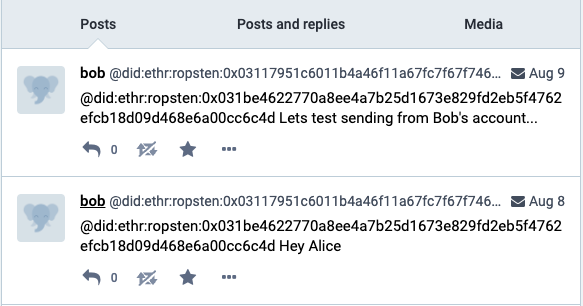
\includegraphics[width=0.8\textwidth]{evaluation/did_toot_2.png}
  \caption{Example of mentioning another user in a \emph{toot} using DIDs.}
  \label{fig:did_toot}
\end{figure}
\chapter{Conclusion}
\label{cha:conclusion}

This thesis presented a design to integrate DIDs and enable DIDComm Messaging v2 into an ActivityPub-based Online Social Network (OSN). The OSN Mastodon was chosen as the representative ActivityPub implementer, where DIDs could be introduced and used to enable DIDComm. 
 The integration of DIDs into ActivityPub was discussed, concluding with the substitution of Mastodon's standard usernames with DIDs. Consequently, a way to preserve the ActivityPub protocol while using DIDComm was explained, resulting in the encapsulation of ActivityPub as the content of a JWM.

Different DID methods were researched in order to find a way to create DIDs and modify the DID documents to include a new verification method and a service endpoint. Tested methods included \emph{did:ion, did:web, did:key} and, \emph{did:bba}. As the selected DID method for the prototype, \emph{did:ethr}, did not support adding RSA keys to a DID document, a custom way was developed with the help of one of the lead developers of the SSI platform provider \emph{Veramo}.
Using the RSA keys and the service endpoints in two DID documents, Mastodon's process to resolve an account in federated communication was modified to partially remove any dependency on centralized third parties and allow a decentralized communication flow when sending a private message. This decentralization process included the following features. First is the ability to send and receive encrypted payload without needing HTTPS for encryption. The second is finding other users based on their DIDs by retrieving their DID documents stored in Ethereum's test network Ropsten instead of using Mastodon's default Webfinger. The DID resolver from the DIF was deployed to achieve the latter. Furthermore, nested JWTs were implemented to provide non-repudiation, message integrity, and encryption using JWM and the JWS and JWE standards.

The proposed design took advantage of most of the features of DIDs and DIDComm. However, it is still not entirely independent of the centralized DNS. In addition, risks and deficiencies were found. For instance, the private key being stored in Mastodons' database and the still present administrators' access to plain-text private messages. Nonetheless, it proved to be a successful implementation of DIDs and DIDComm in a real-world social network. 


% Maybe for other section?
% To test it, two Mastodon instances with these modifications were deployed. Each one had an account with a DID and the respective private key from the DID document. Then, the proposed resolving process was used from one account to find the other. Finally, a private message was sent. During this process, the Activity object was set as the payload of a JWM, signed with the sender's private key, and then encrypted using the receiver's public key retrieved from the DID document. Upon arrival in the receiver's inbox, the JWE was decrypted using the receiver's private key, and the signature was verified using the sender's public key taken from the DID document.




\section{Future Work}
The evaluation has shown that although achieving this thesis's goal, some issues still need to be addressed. For example, the risks imposed by sharing a private key with an ActivityPub server, or Mastodon instance, could be solved using the self-hosted approach of Göndör et al. called \emph{Blade} \cite{inproceedings}. If every user had its own Mastodon server, storing private data would not represent a problem. Nevertheless, this implies a considerable overhead for an average user and goes against the lightweight and easy-to-deploy idea that \emph{Blade} proposes. Alternatively, taking advantage of the marketplace implemented in \emph{Blade}, a module for ActivityPub that can interact with a Mastodon instance while keeping private data under the user's control, could prove to be a better option. 

Furthermore, a registration process that takes advantage of the \emph{authentication} property of a DID document has yet to be implemented. Spruce\footnote{https://www.spruceid.com/} is working on a similar idea, where a user is able to \emph{sign in} to a service using their Ethereum-based \emph{ENS} domain. 

Finally, further development for the DID-based Mastodon prototype is intended. The goal is to be able to participate in the federation while still supporting DIDs by adding backward compatibility. In this manner, DIDs can be introduced to Mastodon and promote their further adoption. Following this idea, a DIDComm endpoint will be adapted so that users can send private messages, following the design proposed in this thesis.

%--------------------------------------------------------------
% TABLES, FIGURES, BIBLOGRAPHY AND APPENDICES
%--------------------------------------------------------------
\backmatter

% Lists of tables and figures
\listoftables
\listoffigures

% Bibliography
\setwidesite{}						% Set page to be wider for bibliography
\markboth{Bibliography}{bibliography}
\label{cha:bibliography}
\bibliographystyle{IEEEtran}
\bibliography{bibliography.bib}

% Use following to separate online (websites) and offline (books, papers) sources
%\printbibliography[heading=offline,filter=offline]
%\printbibliography[heading=online,filter=online]

\begin{appendices}
	\chapter{Appendix: Listings}

\lstset{style=JSONStyle}
\begin{lstlisting}[language=PHP, caption=Mastodon extended version of ActivityPub's actor object of user bob@mastodon.social, label=fig:mastodon_actor_object, float=ht]
{
    "@context": [
        "https://www.w3.org/ns/activitystreams",
    ],
    "id": "https://mastodon.social/users/bob",
    "type": "Person",
    "following": "https://mastodon.social/users/bob/following",
    "followers": "https://mastodon.social/users/bob/followers",
    "inbox": "https://mastodon.social/users/bob/inbox",
    "outbox": "https://mastodon.social/users/bob/outbox",
    "featured": "https://mastodon.social/users/bob/collections/featured",
    "featuredTags": "https://mastodon.social/users/bob/collections/tags",
    "preferredUsername": "bob",
    "name": "Bob",
    "summary": "",
    "url": "https://mastodon.social/@bob",
    "manuallyApprovesFollowers": false,
    "discoverable": false,
    "published": "2022-01-18T00:00:00Z",
    "devices": "https://mastodon.social/users/bob/collections/devices",
    "publicKey": {
        "id": "https://mastodon.social/users/bob#main-key",
        "owner": "https://mastodon.social/users/bob",
        "publicKeyPem": "-----BEGIN PUBLIC KEY-----\n..."
    },
    "tag": [],
    "attachment": [],
    "endpoints": {
        "sharedInbox": "https://mastodon.social/inbox"
    },
    "icon": {
        "type": "Image",
        "mediaType": "image/jpeg",
        "url": "https://files.mastodon.social/accounts/avatars/107.jpg"
    }
}
\end{lstlisting}


\lstset{style=JSONStyle}
\begin{lstlisting}[language=PHP, caption=Example of encrypted message using Mastodon's E2EE API and extended JSON-LD vocabulary, label=appendix:e2e, float=ht]
  {
    "@context": [
      "https://www.w3.org/ns/activitystreams",
      {
        "toot": "http://joinmastodon.org/ns#",
        "Device": "toot:Device",
        "Ed25519Signature": "toot:Ed25519Signature",
        "Ed25519Key": "toot:Ed25519Key",
        "Curve25519Key": "toot:Curve25519Key",
        "EncryptedMessage": "toot:EncryptedMessage",
        "publicKeyBase64": "toot:publicKeyBase64",
        "deviceId": "toot:deviceId",
        "claim": {
          "@type": "@id",
          "@id": "toot:claim"
        },
        "fingerprintKey": {
          "@type": "@id",
          "@id": "toot:fingerprintKey"
        },
        "identityKey": {...},
        "devices": {...},
        "messageFranking": "toot:messageFranking",
        "messageType": "toot:messageType",
        "cipherText": "toot:cipherText"
      }
    ],
    "id": "http://localhost:3000/f41c9aae-92fc-48bf-8d87-0606197f340a",
    "type": "Create",
    "actor": "http://localhost:3000/users/admin",
    "to": "http://localhost:3000/users/velda_moriette0",
    "object": {
      "type": "EncryptedMessage",
      "messageType": 0,
      "cipherText": "AwogNcm0y1HR42K07iyNs37uTlQ7jrX3n7...",
      "digest": {
        "type": "Digest",
        "digestAlgorithm": "http://www.w3.org/2000/09/xmldsig#hmac-sha256",
        "digestValue": "5f6ad31acd64995483d75..."
      },
      "messageFranking": "...",
      "attributedTo": {
        "type": "Device",
        "deviceId": "11119"
      },
      "to": {
        "type": "Device",
        "deviceId": "11876"
      }
    }
  }
\end{lstlisting}

\lstset{style=JSONStyle}
\begin{lstlisting}[language=PHP, caption=DID Document for Alicecreated with the \emph{did:ethr} DID method. It includes an RSA public key and a service that points to her profile URL in the Mastodon instance \emph{lisztos.com}, label=lst:alice_ethr_doc, float=ht]
  {
    "@context": [
      "https://www.w3.org/ns/did/v1",
      "https://w3id.org/security/suites/secp256k1recovery-2020/v2"
    ],
    "id": "did:ethr:ropsten:0x031be4622770a8ee4a7b25d1673e829fd2eb5f4762efcb18d09d468e6a00cc6c4d",
    "verificationMethod": [
      {
        "id": "did:ethr:ropsten:0x031be4622770a8ee4a7b25d1673e829fd2eb5f4762efcb18d09d468e6a00cc6c4d#controller",
        "type": "EcdsaSecp256k1RecoveryMethod2020",
        "controller": "did:ethr:ropsten:0x031be4622770a8ee4a7b25d1673e829fd2eb5f4762efcb18d09d468e6a00cc6c4d",
        "blockchainAccountId": "eip155:3:0x577361D41748c83ab328E90a51054712Fe49e211"
      },
      {
        "id": "did:ethr:ropsten:0x031be4622770a8ee4a7b25d1673e829fd2eb5f4762efcb18d09d468e6a00cc6c4d#delegate-1",
        "type": "RSAVerificationKey2018",
        "controller": "did:ethr:ropsten:0x031be4622770a8ee4a7b25d1673e829fd2eb5f4762efcb18d09d468e6a00cc6c4d",
        "publicKeyPem": "-----BEGIN PUBLIC KEY-----\nMIIBIjANBgkqhkiG9w0BAQEFA...npUZV+Q1FdWLiuFlKAwDt3DiD3\nNSz2b27Iga7wTSCoQ/DAhFAZ8KH8uCMrioIWFSKuYRgFOysbDfTT9Kpha8ST8K/H\nTQIDAQAB\n-----END PUBLIC KEY-----\n"
      }
    ],
    "authentication": [...],
    "assertionMethod": [...],
    "service": [
      {
        "id": "did:ethr:ropsten:0x031be4622770a8ee4a7b25d1673e829fd2eb5f4762efcb18d09d468e6a00cc6c4d#service-1",
        "type": "ActivityPub",
        "serviceEndpoint": "http://lisztos.com/users/did:ethr:ropsten:0x031be4622770a8ee4a7b25d1673e829fd2eb5f4762efcb18d09d468e6a00cc6c4d"
      }
    ]
  }
\end{lstlisting}
	% \input{content/99_appendices/a02_listings}
	% \input{content/99_appendices/a03_listings}
\end{appendices}

\end{document}
